% $Header: /cvsroot/latex-beamer/latex-beamer/solutions/generic-talks/generic-ornate-15min-45min.en.tex,v 1.5 2007/01/28 20:48:23 tantau Exp $

\documentclass[12pt]{beamer}
%\documentclass[12pt,handout]{beamer}

% This file is a solution template for:

% - Giving a talk on some subject.
% - The talk is between 15min and 45min long.
% - Style is ornate.



% Copyright 2004 by Till Tantau <tantau@users.sourceforge.net>.
%
% In principle, this file can be redistributed and/or modified under
% the terms of the GNU Public License, version 2.
%
% However, this file is supposed to be a template to be modified
% for your own needs. For this reason, if you use this file as a
% template and not specifically distribute it as part of a another
% package/program, I grant the extra permission to freely copy and
% modify this file as you see fit and even to delete this copyright
% notice.


\mode<presentation>
{
  \usetheme{default}
  % or ...

  \setbeamercovered{transparent}
  % or whatever (possibly just delete it)
}
\setbeamertemplate{navigation symbols}{}%remove navigation symbols


\usepackage[english]{babel}
% or whatever

\usepackage[latin1]{inputenc}
% or whatever

\usepackage{times}
\usepackage{sansmathfonts}
\usepackage[T1]{fontenc}
% Or whatever. Note that the encoding and the font should match. If T1
% does not look nice, try deleting the line with the fontenc.


\title%[Short Paper Title] % (optional, use only with long paper titles)
{}

\subtitle
{} % (optional)

\author%[Author, Another] (optional, use only with lots of authors)
{Ben Holder}%{F.~Author\inst{1} \and S.~Another\inst{2}}
% - Use the \inst{?} command only if the authors have different
%   affiliation.

%\institute[Universities of Somewhere and Elsewhere] % (optional, but mostly needed)
%{
%  \inst{1}%
%  Department of Computer Science\\
%  University of Somewhere
%  \and
%  \inst{2}%
%  Department of Theoretical Philosophy\\
%  University of Elsewhere}
%% - Use the \inst command only if there are several affiliations.
%% - Keep it simple, no one is interested in your street address.

\date%[Short Occasion] % (optional)
{}

\subject{Talks}
% This is only inserted into the PDF information catalog. Can be left
% out.



% If you have a file called "university-logo-filename.xxx", where xxx
% is a graphic format that can be processed by latex or pdflatex,
% resp., then you can add a logo as follows:

% \pgfdeclareimage[height=0.5cm]{university-logo}{university-logo-filename}
% \logo{\pgfuseimage{university-logo}}



% Delete this, if you do not want the table of contents to pop up at
% the beginning of each subsection:
%\AtBeginSubsection[]
%{
%  \begin{frame}<beamer>{Outline}
%    \tableofcontents[currentsection,currentsubsection]
%  \end{frame}
%}


% If you wish to uncover everything in a step-wise fashion, uncomment
% the following command:

%\beamerdefaultoverlayspecification{<+->}

\usepackage{enumerate}
\usepackage{amsmath}
\usepackage{amssymb}
\usepackage[amssymb]{SIunits}
\usepackage{url}
\usepackage{hyperref}
\usepackage[normalem]{ulem}


\setbeamercovered{invisible}

\hypersetup{
    colorlinks=true,     % false: boxed links; true: colored links
    linkcolor=red,       % color of internal links
    citecolor=blue,      % color of links to bibliography
    filecolor=blue,      % color of file links
    urlcolor=blue        % color of external links
}


\begin{document}

%\begin{frame}
%  \titlepage
%\end{frame}

%%%%%%%%%%%%%%%%%%%%%%%%%%%%%%%%%%%%%%
\begin{frame}{Announcements}
	%
	\begin{itemize}
	\addtolength{\itemsep}{0.5\baselineskip}
	\item[]{\bf Today (Lecture)}: Contemporary Climate Change: Is the climate changing and how do we know what we know?
	\item[]{\bf Tomorrow (Lab)}: Estimating the ``Global Average Temperature''
	\item[]{\bf Thursday (Discussion)}]: Local Weather Variations and Exploring IPCC Data
	\item Next Week: Energy and Equilibrium
		%
	\end{itemize}
	\vfill
	{\small Today's lecture is adapted from Nadir Jeevanjee's ``Science on Tap'' bar talk \href{https://nadirjeevanjee.com/lectures.html}{\em How do we know what we know?}}

\begin{center}
%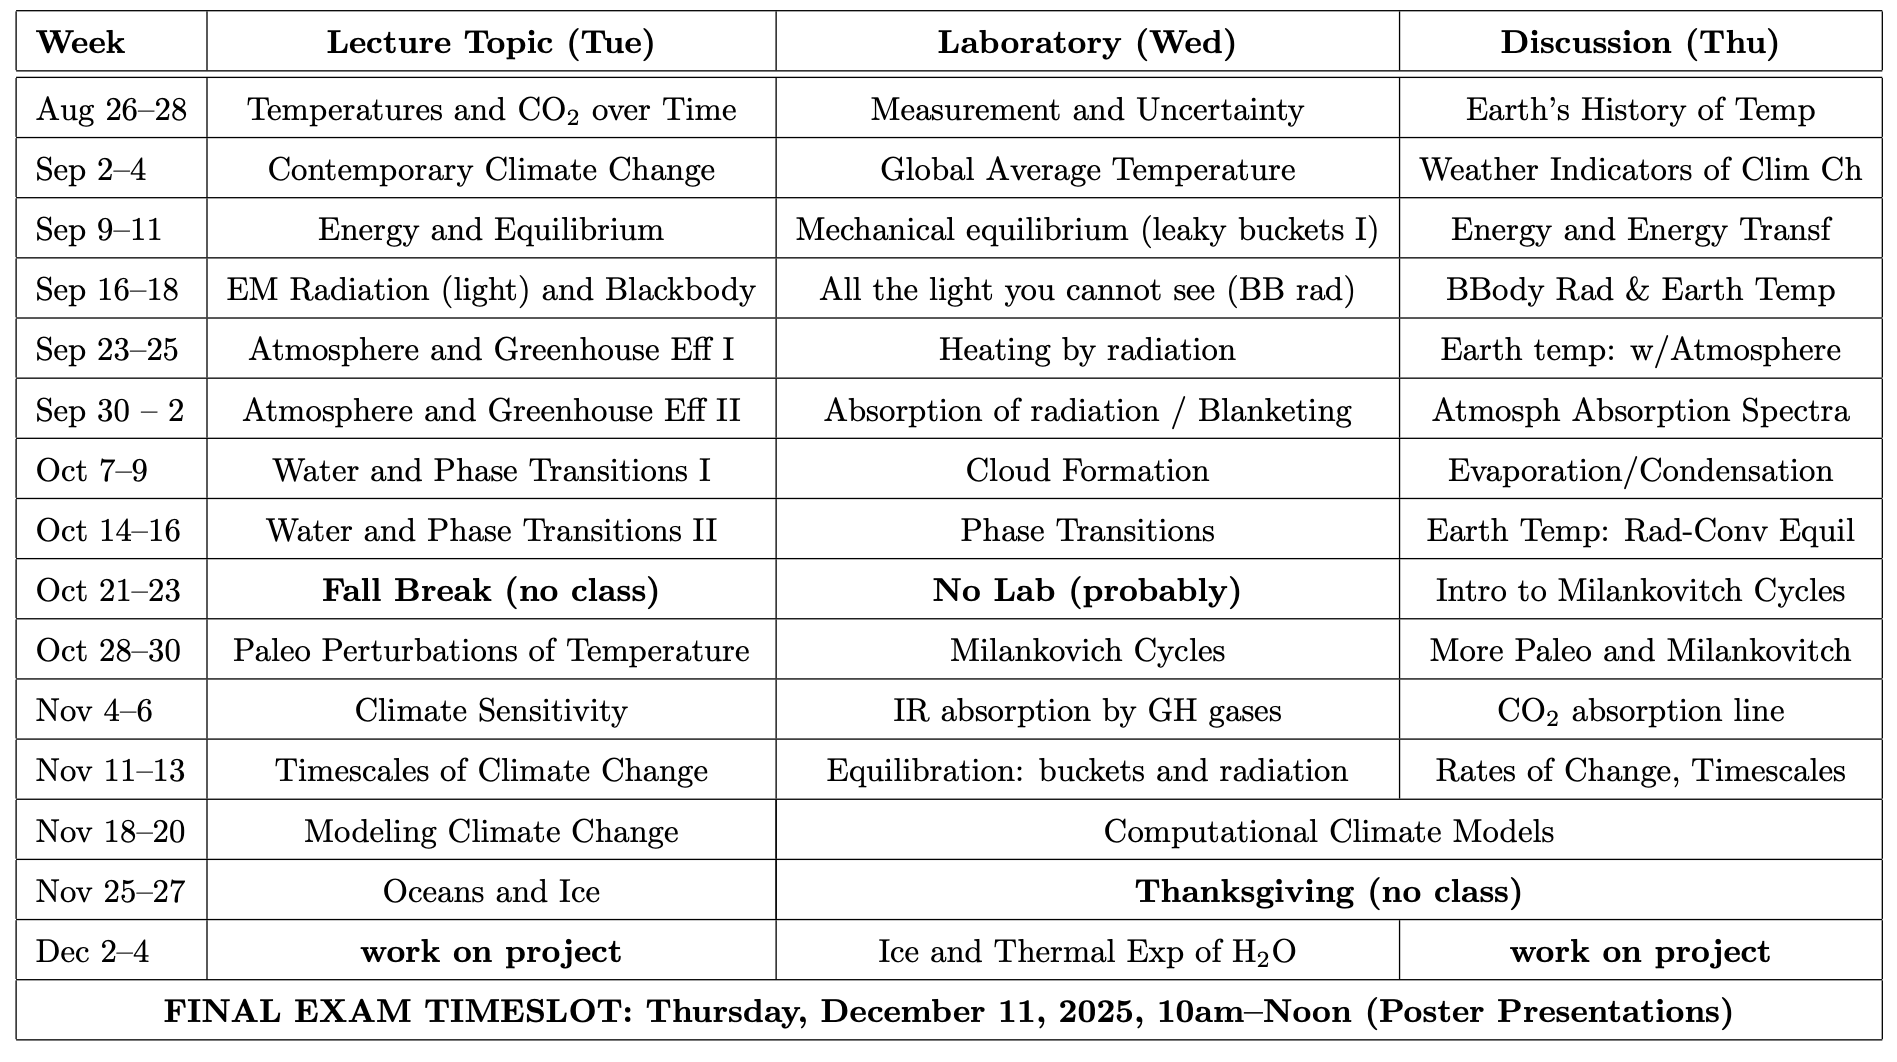
\includegraphics[width=0.8\textwidth]{images/calendar-F2025}
\end{center}

\end{frame}
%%%%%%%%%%%%%%%%%%%%%%%%%%%%%%%%%%%%%%
\begin{frame}{Today's Reading Quiz (3 min)}

On your own sheet of paper\ldots

\vspace{2cm}

\begin{center}
Discuss temperatures in Houston vs.\ Amarillo, TX, including the meaning and use of {\em temperature anomaly}.
\end{center}

\vspace{2cm}

Turn in to Blackboard as scanned pdf.

\end{frame}
%%%%%%%%%%%%%%%%%%%%%%%%%%%%%%%%%%%%%%
\begin{frame}{Temperature Anomalies}



\begin{center}
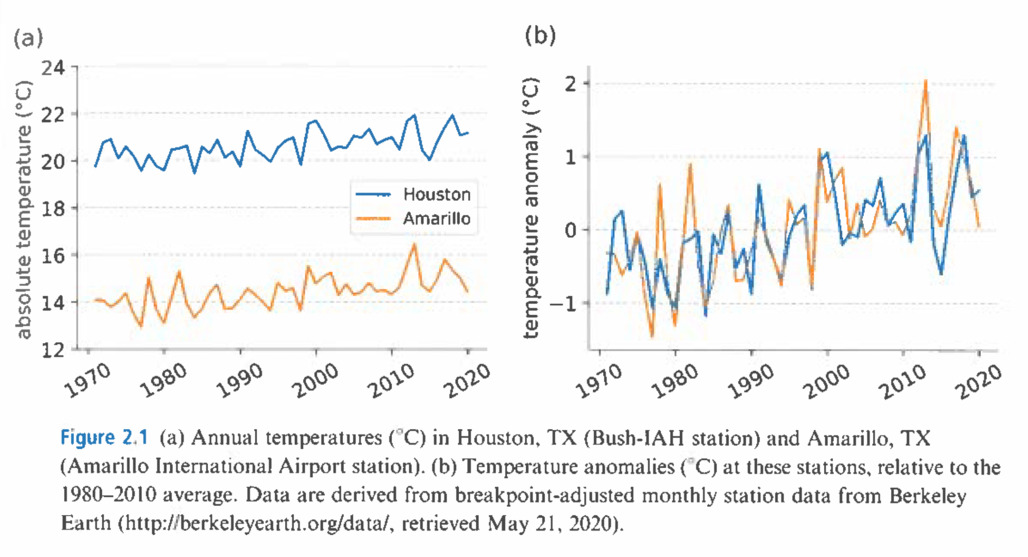
\includegraphics[width=0.8\textwidth]{images/dessler_amarillo-vs-houston_fig2-1.jpg}
\end{center}

\begin{itemize}
\item Average annual temperatures are significantly different at the gulf coast and the border with Oklahoma!
\item Temperature anomalies are taken in reference to some chosen average value (here: 1980--2010).
\item That reference point is always {\em local}: Each location has an anomaly with respect to its average reference point.
\end{itemize}

\end{frame}
%%%%%%%%%%%%%%%%%%%%%%%%%%%%%%%%%%%%%%
\begin{frame}{Is the Climate Changing?}



\begin{center}
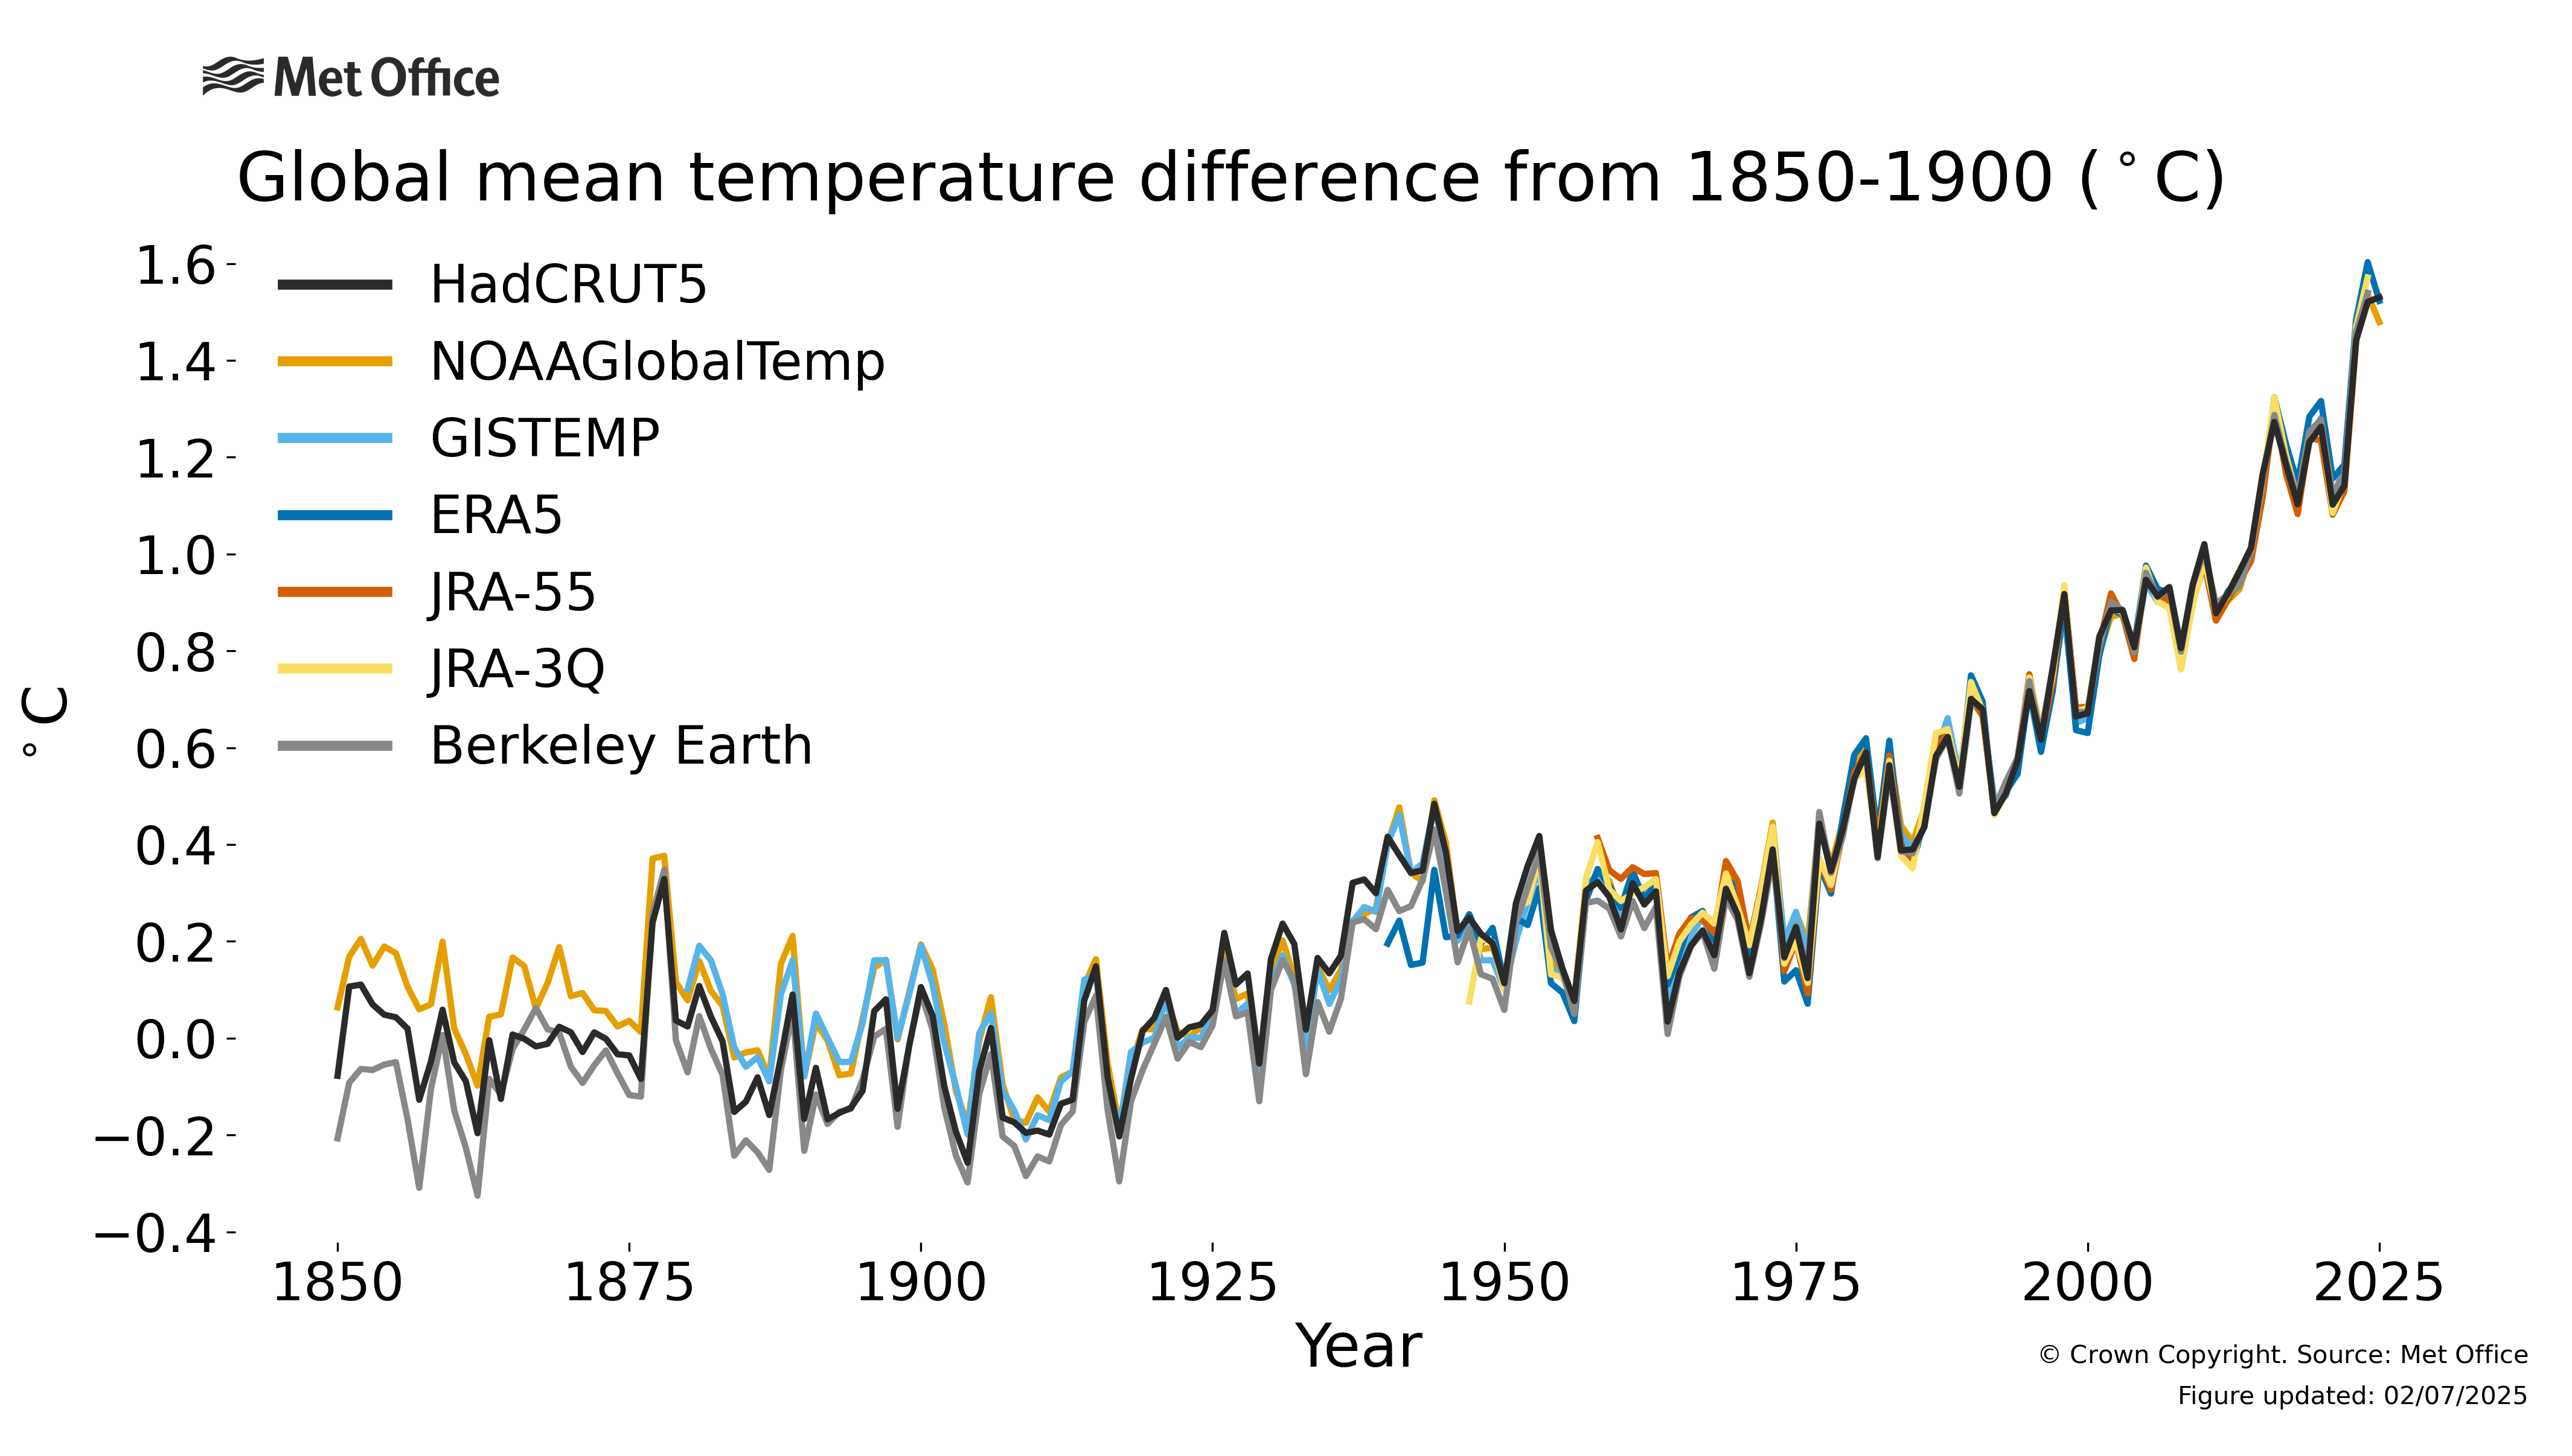
\includegraphics[width=0.7\textwidth]{images/global-average-temperature_met-office_2025-09}
\end{center}
%
\begin{itemize}
\item What can we say about uncertainty from instruments/methods over time? (Compare independent measurements)
\item What can we say about natural variability?
\item Is there a {\em change} in global average temperature from 1850--1975?  from 1975--2025?
\end{itemize}
%

\end{frame}
%%%%%%%%%%%%%%%%%%%%%%%%%%%%%%%%%%%%%%
\begin{frame}{More on uncertainty from natural variation}

\begin{center}
\begin{minipage}{\textwidth}
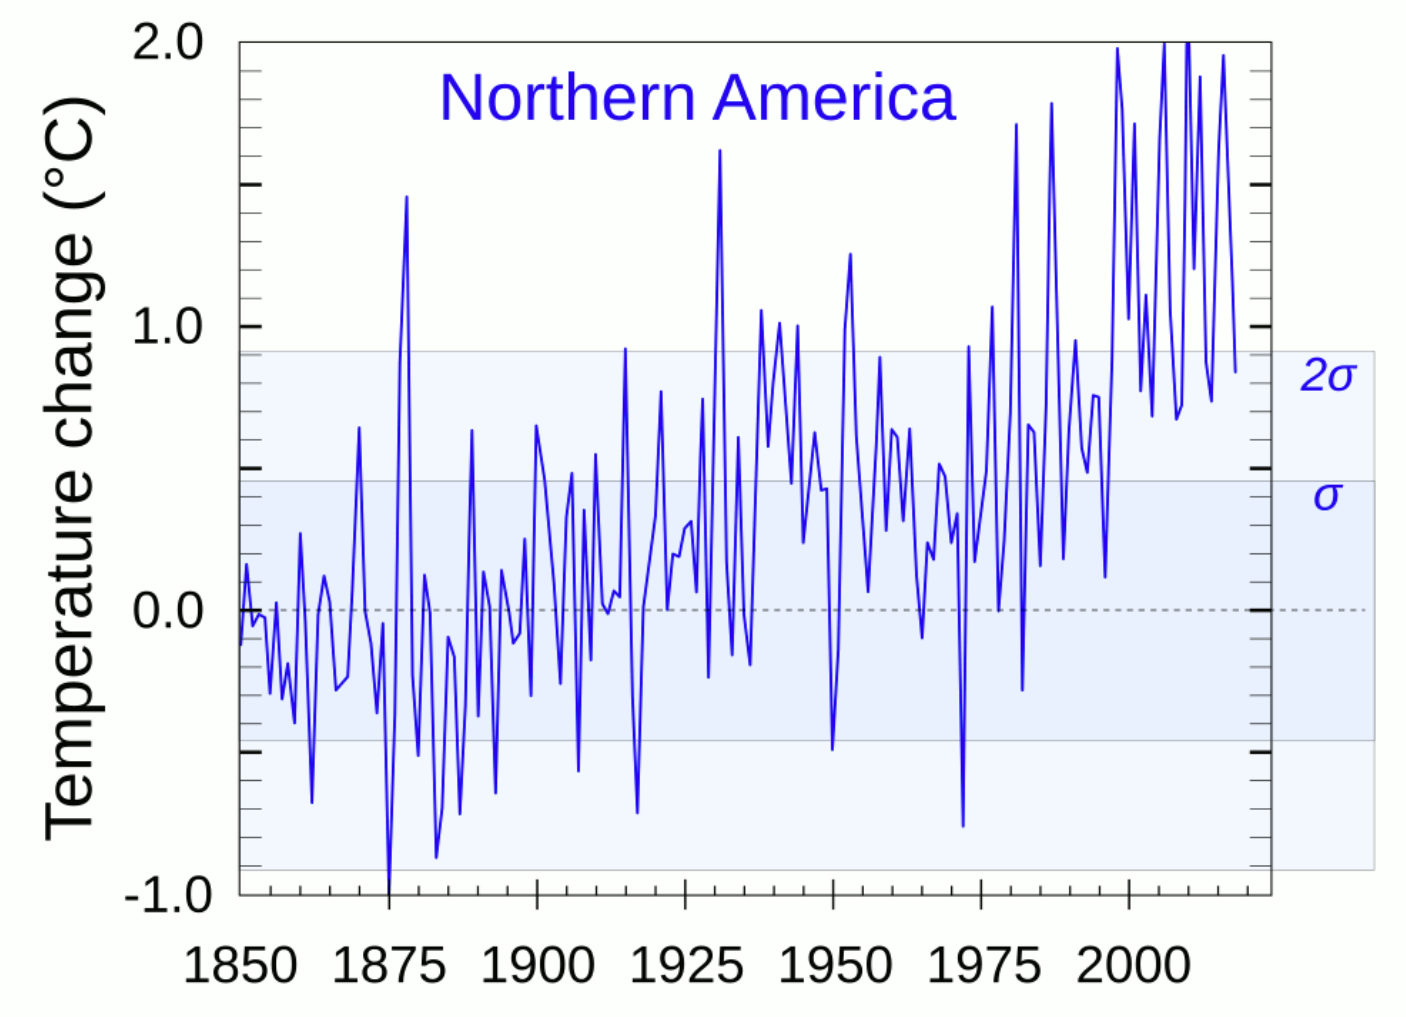
\includegraphics[width=0.48\textwidth]{images/temperature-and-variability_north-america.png}%
\hfill %
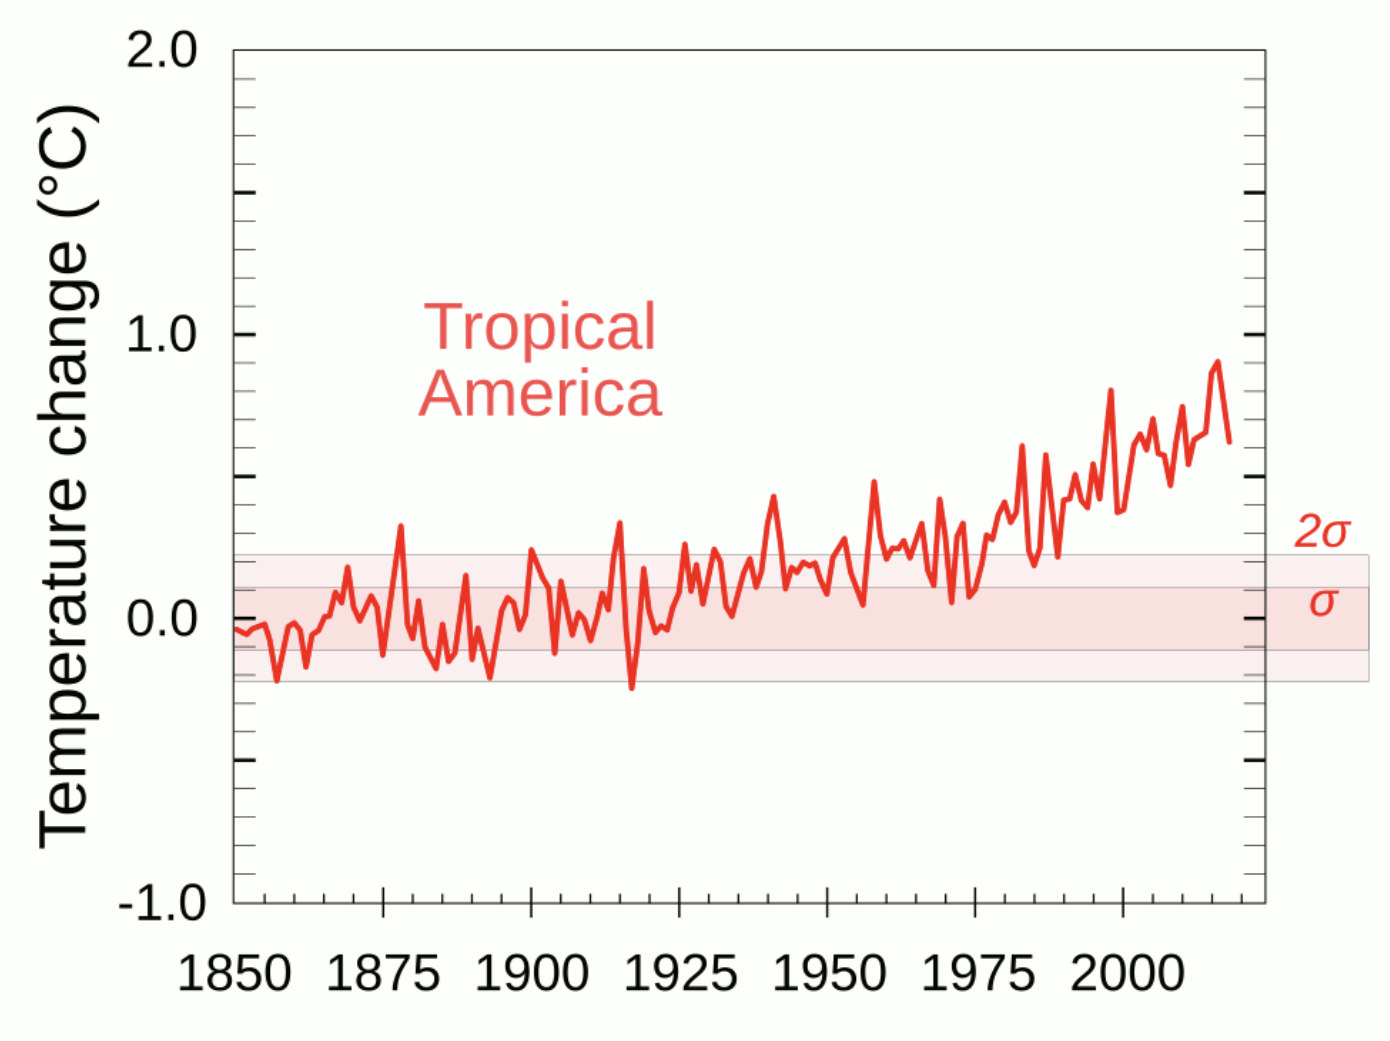
\includegraphics[width=0.48\textwidth]{images/temperature-and-variability_tropical-americas.png}
\makebox[\textwidth][r]{
\tiny From \href{https://en.wikipedia.org/wiki/File:20200509_Emergence_of_temperatures_from_range_of_normal_historical_variability_-_tropical_vs_northern_Americas_(Hawkins).gif}{{Wikimedia: Emergence of temperatures\ldots}}
}
\end{minipage}
\end{center}
%

%
\begin{itemize}
\item Note differences in two sets of measurements: in variation, and magnitude of change.
\item  Uncertainty (here: from observed natural variation) gives us a {\em standard deviation}.  Departure from that range indicates the identification of an effect.
\end{itemize}
%

\end{frame}
%%%%%%%%%%%%%%%%%%%%%%%%%%%%%%%%%%%%%%
\begin{frame}{Perhaps not enough time to see variations?}

{\small Last week in Discussion we saw large variations in temperature over the history of Earth:}
%
\begin{center}
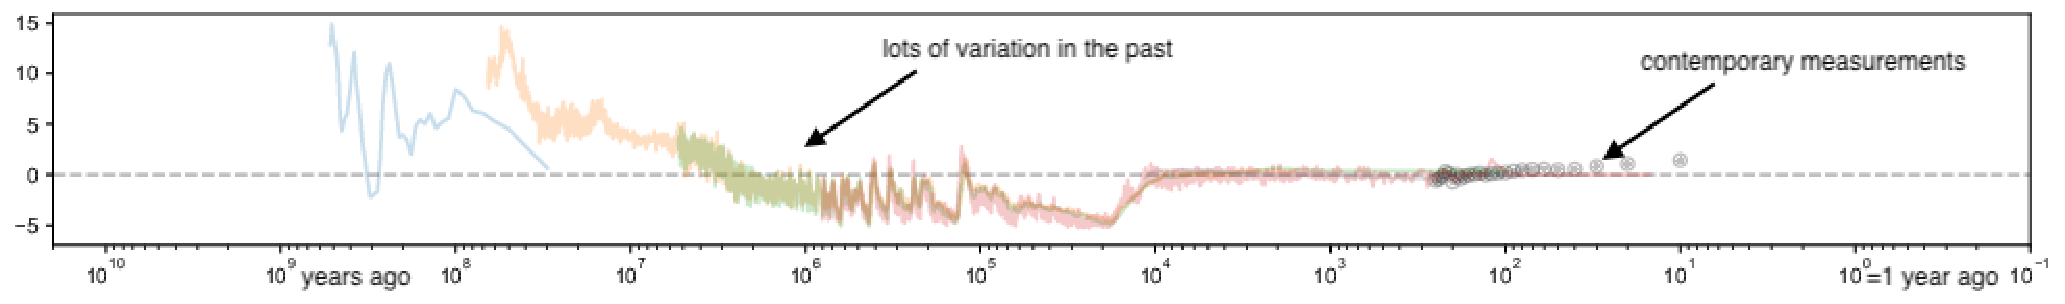
\includegraphics[width=\textwidth]{images/row5_log-all_marked-up.pdf}
\end{center}
%
{\small Particularly in the ice-ages/interglacials (past one million years):}
%
\begin{center}
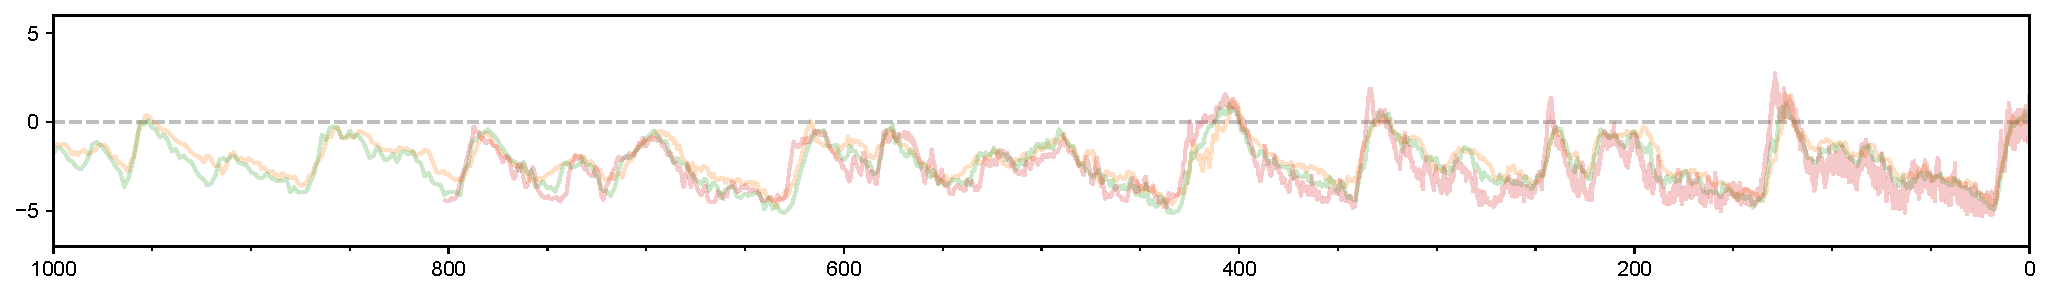
\includegraphics[width=\textwidth]{images/row3_1Mya.pdf}
\end{center}
%
{\small But look at the time {\em since} the last ice age (25,000 ya):}
%
\begin{center}
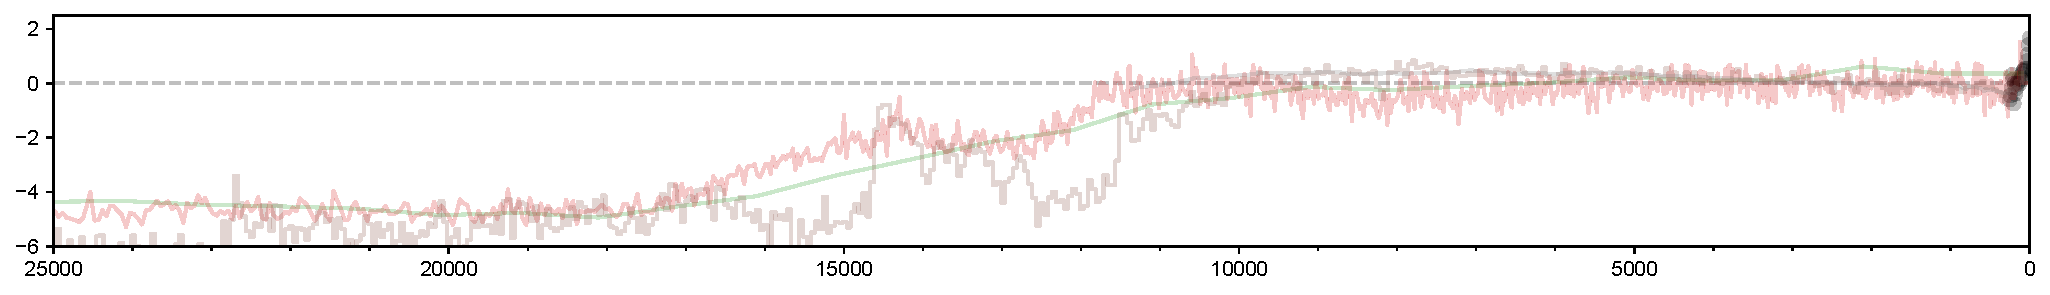
\includegraphics[width=\textwidth]{images/row4_25kya.pdf}
\end{center}
%

\end{frame}
%%%%%%%%%%%%%%%%%%%%%%%%%%%%%%%%%%%%%%
\begin{frame}{Why is the temperature increasing?}

\begin{center}
\begin{minipage}{0.4\textwidth}
\vspace{0pt}
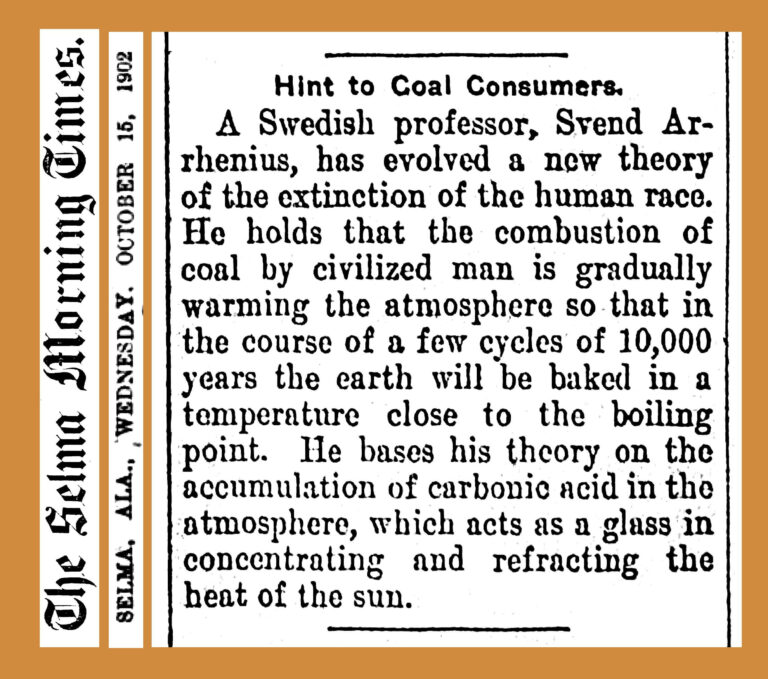
\includegraphics[width=0.9\textwidth]{images/svante-arrhenius_coal-and-warming_1902.jpg}\\
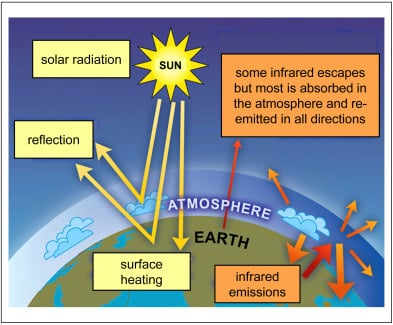
\includegraphics[width=0.9\textwidth]{images/greenhouse-effect_IPCC-2007}
%\makebox[\textwidth][r]{
%\tiny From \href{https://en.wikipedia.org/wiki/File:20200509_Emergence_of_temperatures_from_range_of_normal_historical_variability_-_tropical_vs_northern_Americas_(Hawkins).gif}{{Wikimedia: Emergence of temperatures\ldots}}
%}
\end{minipage} %
\hfill %
\begin{minipage}{0.5\textwidth}
\vspace{0pt}
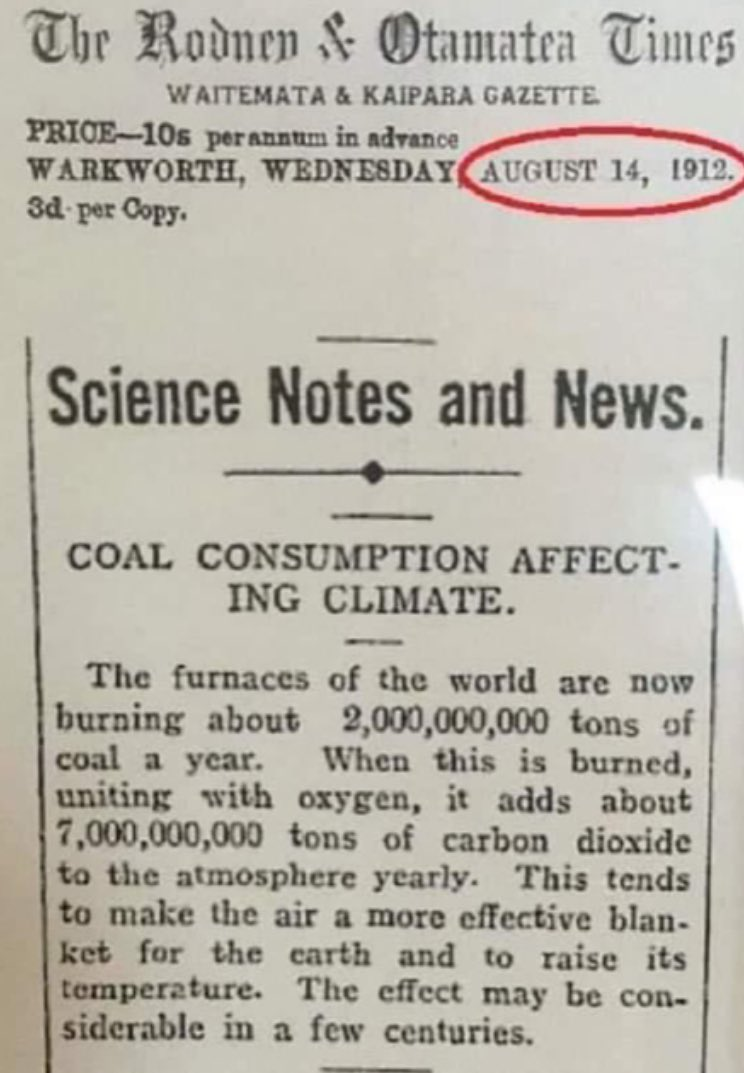
\includegraphics[width=0.8\textwidth]{images/rodnen-otamatea-times_climate-change_1912.jpeg}
\end{minipage}
\end{center}
%

% Arrhenius won 1903 Nobel Prize in Chemistry.  "in recognition of the extraordinary services he has rendered to the advancement of chemistry by his electrolytic theory of dissociation"
% predicted that doubling CO2 would increase global temperature by 4 degrees C

\begin{itemize}
\item Answer: primarily due to the ``greenhouse effect'' from ``greenhouse gases'' ($\text{CO}_2$, methane)
\end{itemize}

\end{frame}
%%%%%%%%%%%%%%%%%%%%%%%%%%%%%%%%%%%%%%
\begin{frame}{How do we know that $\text{CO}_2$ is increasing?}

\begin{center}
\begin{minipage}{0.62\textwidth}
\vspace{0pt}
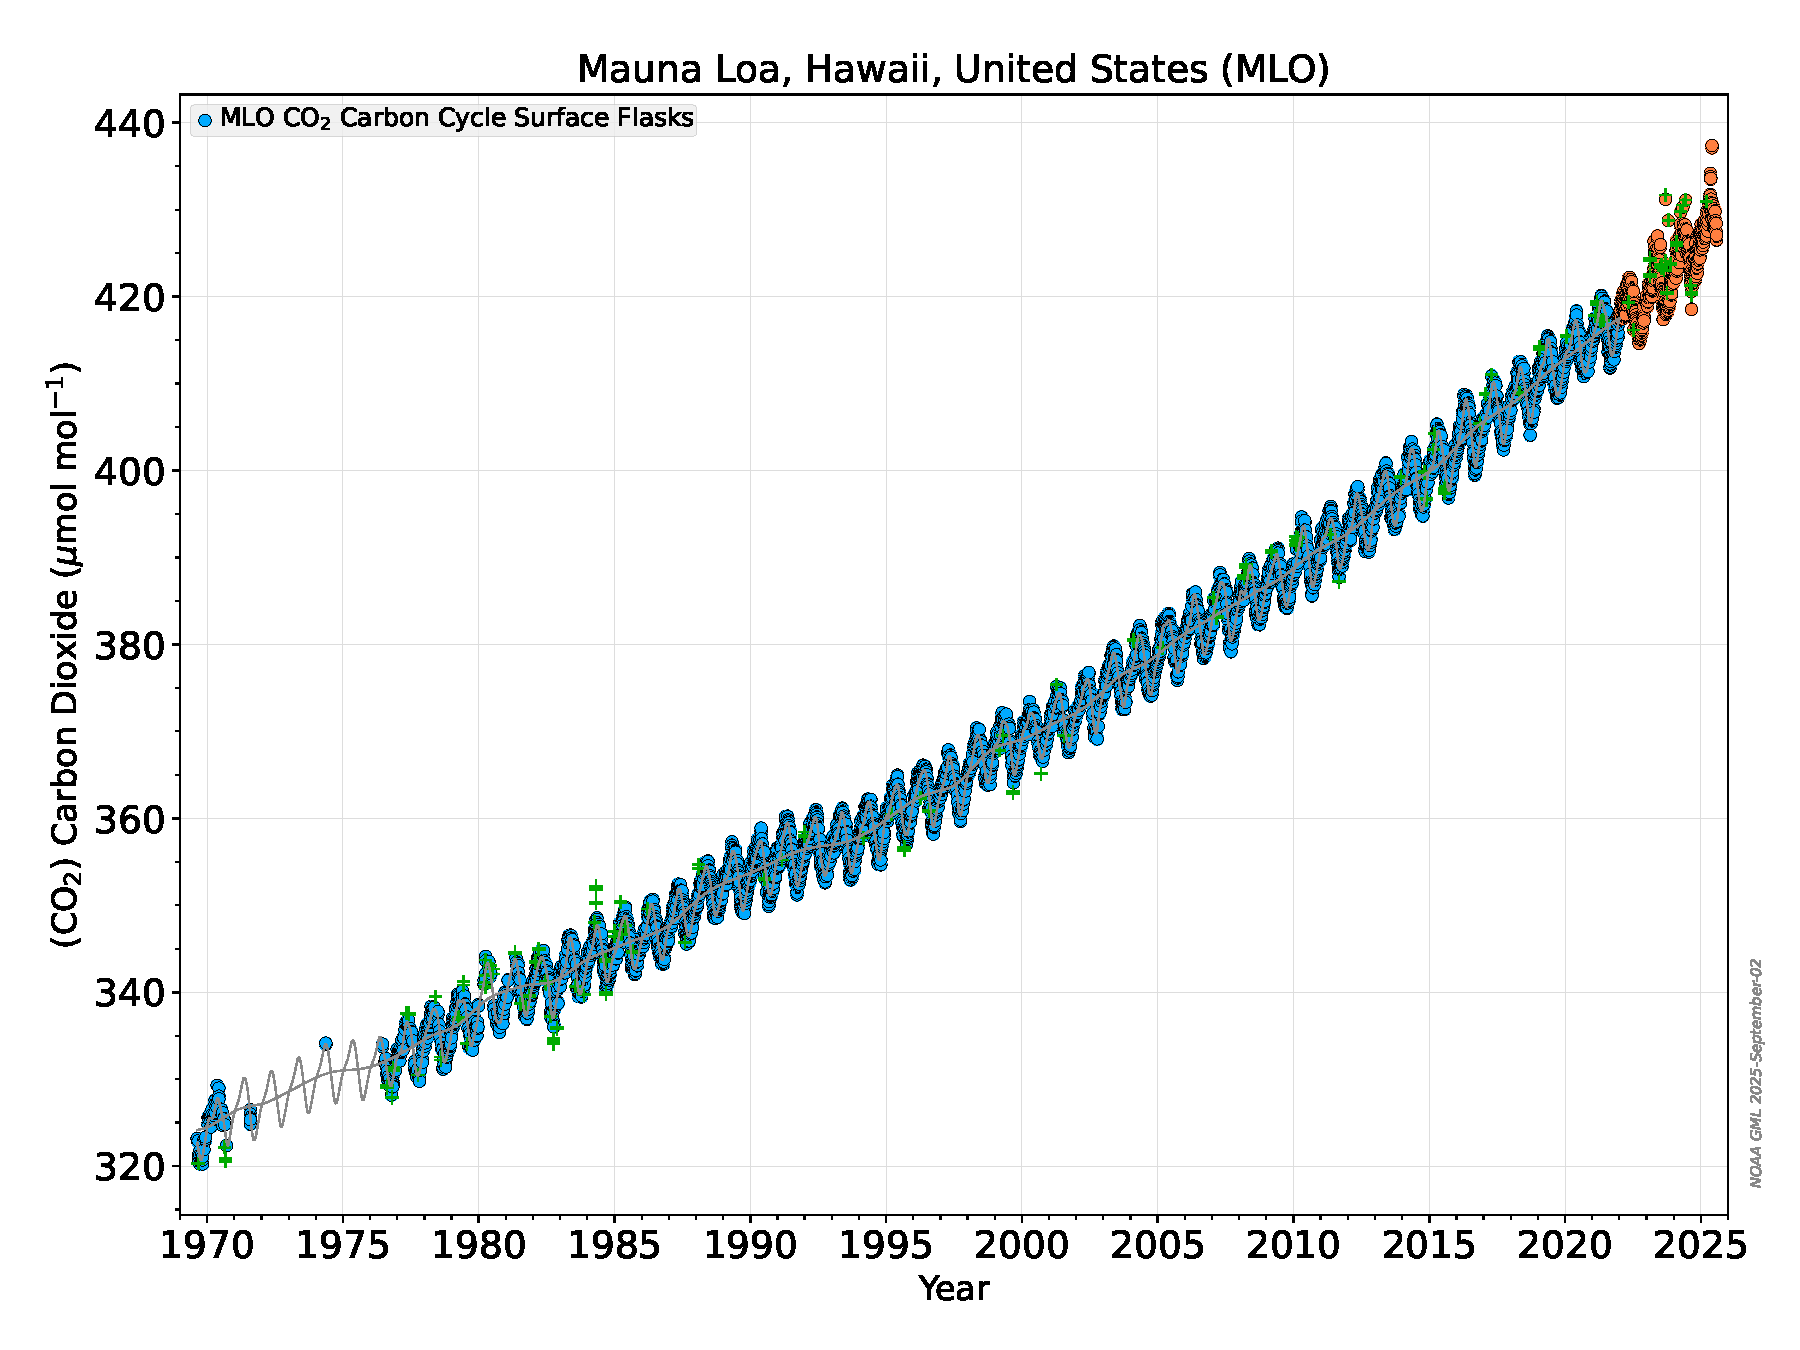
\includegraphics[width=\textwidth]{images/mauna-loa-data_2025-09-01.pdf}
\end{minipage} %
\hfill %
\begin{minipage}{0.35\textwidth}
\vspace{0pt}
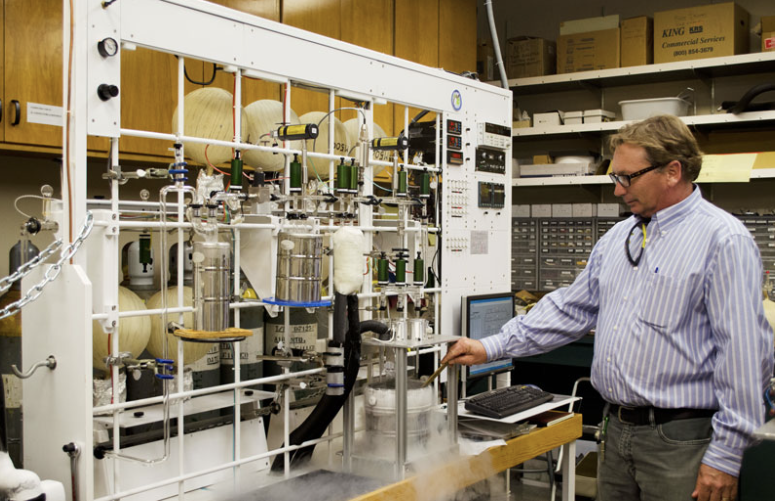
\includegraphics[width=\textwidth]{images/co2_bottling.png}
\end{minipage}
\end{center}
%

% Arrhenius won 1903 Nobel Prize in Chemistry.  "in recognition of the extraordinary services he has rendered to the advancement of chemistry by his electrolytic theory of dissociation"
% predicted that doubling CO2 would increase global temperature by 4 degrees C

\begin{itemize}
\item Answer: We have been measuring for over 50 years!
\end{itemize}

\end{frame}
%%%%%%%%%%%%%%%%%%%%%%%%%%%%%%%%%%%%%%
\begin{frame}{How do we know that $\text{CO}_2$ is increasing?}

\begin{center}
\begin{minipage}{0.62\textwidth}
\vspace{0pt}
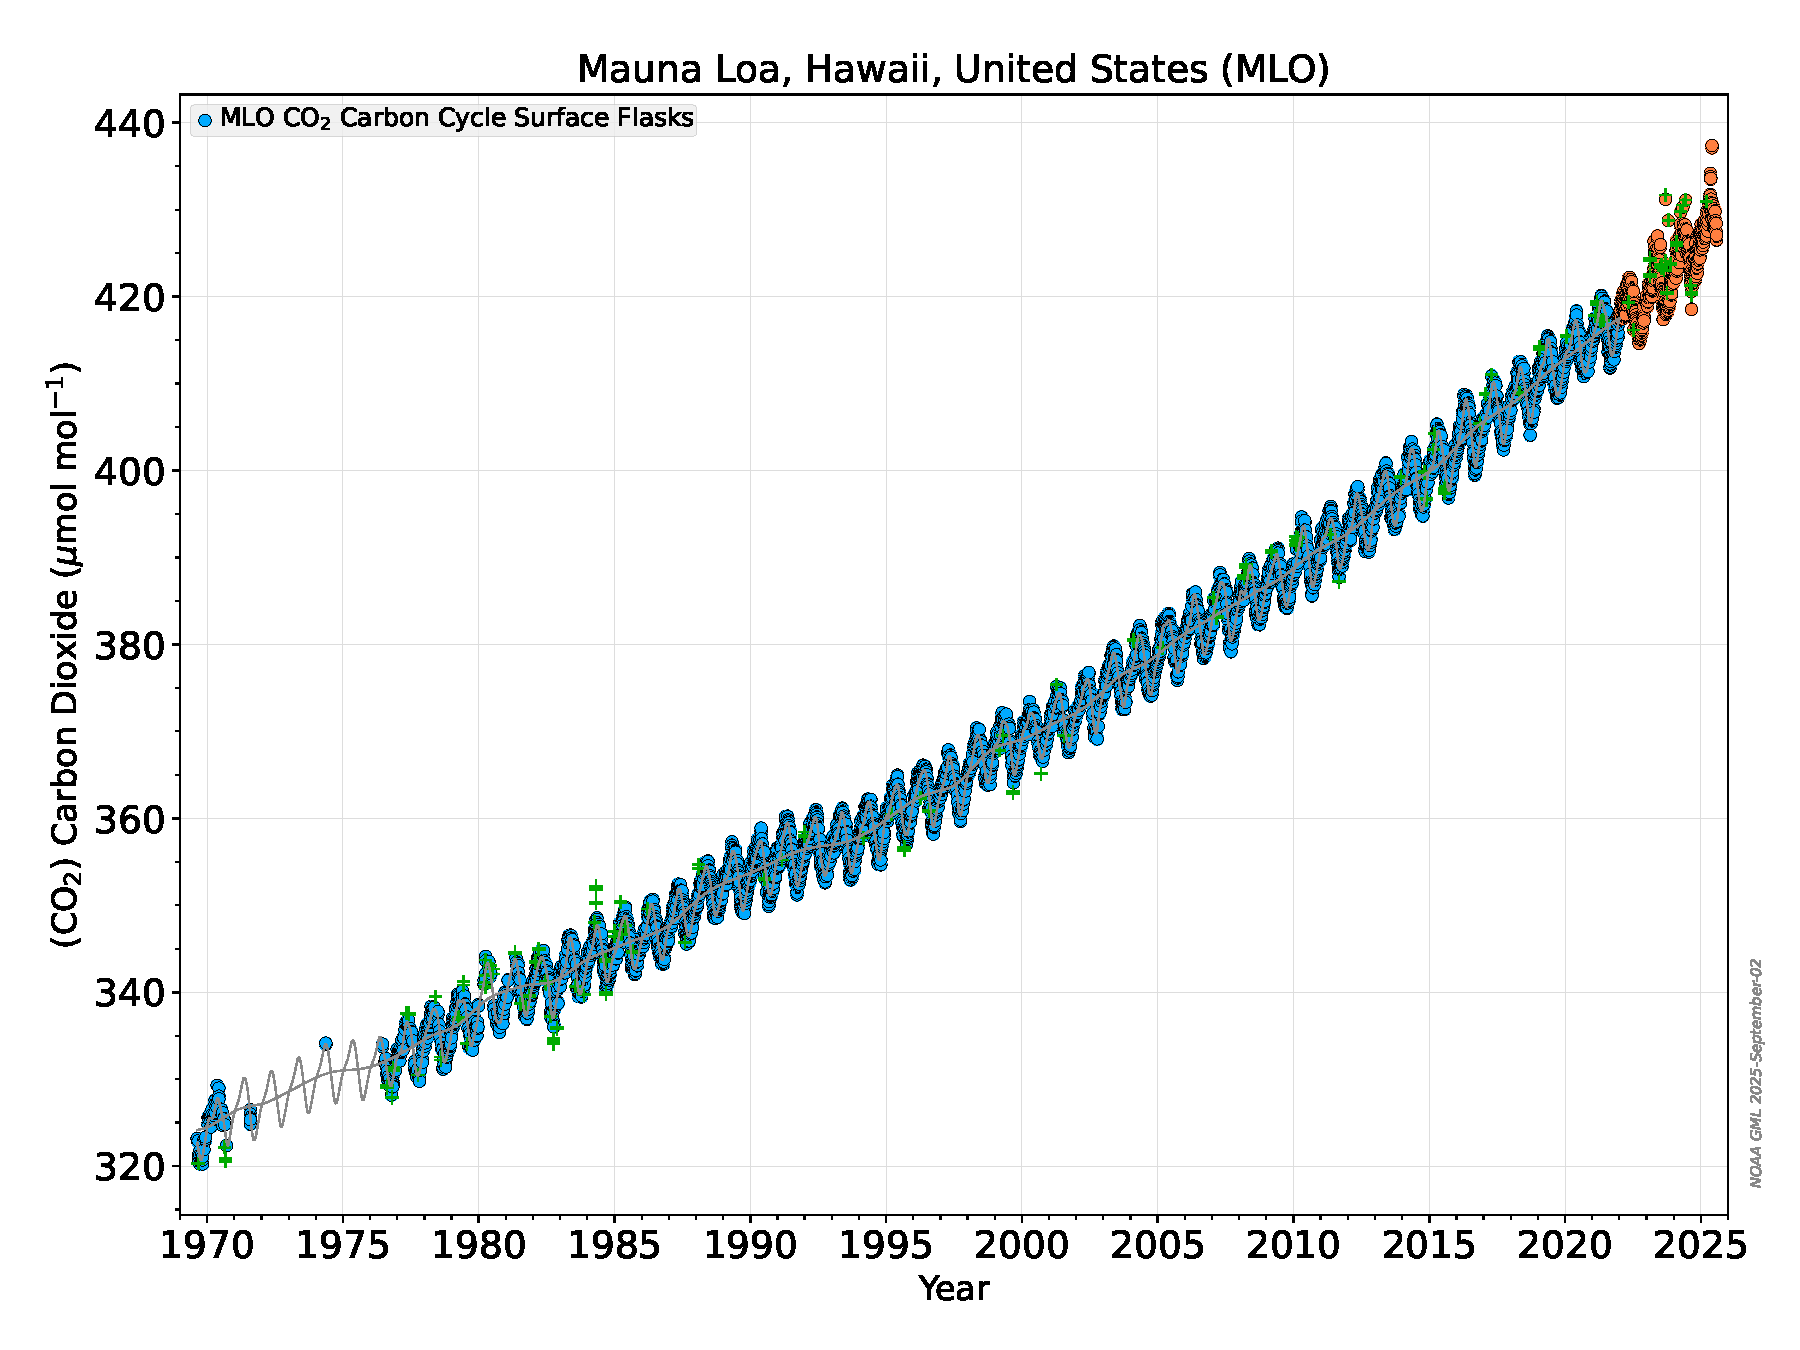
\includegraphics[width=0.9\textwidth]{images/mauna-loa-data_2025-09-01.pdf}
\end{minipage} %
\hfill %
\begin{minipage}{0.35\textwidth}
\vspace{0pt}
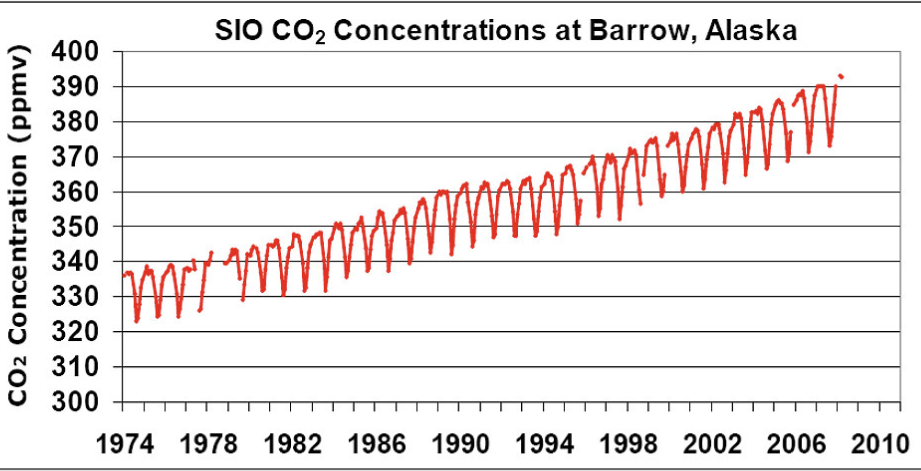
\includegraphics[width=\textwidth]{images/co2_alaska.png}\\[12pt]
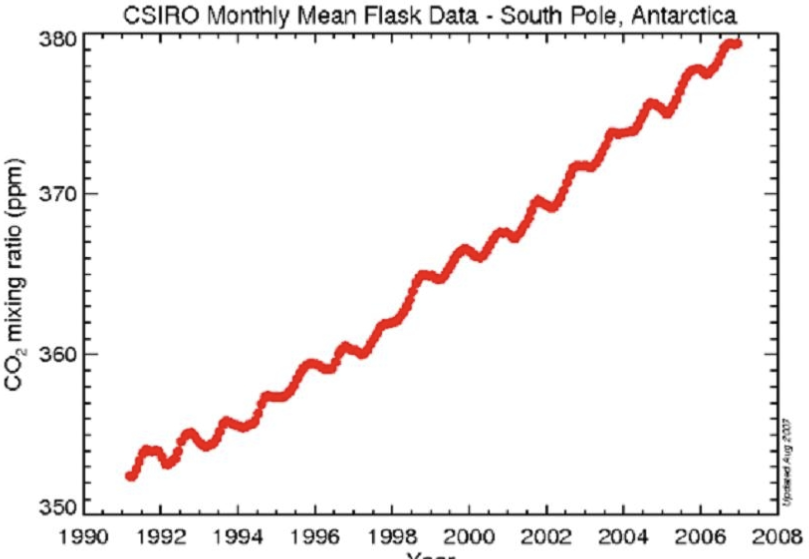
\includegraphics[width=\textwidth]{images/co2_antartica.png}
\end{minipage}
\end{center}
%


\begin{itemize}
\item Each station shows approximately an 1--2 parts per million (ppm) increase in atmospheric $\text{CO}_2$ per year.
\end{itemize}

{\small (What is ``ppm'' anyway?  What part of the air is this?)}
\end{frame}
%%%%%%%%%%%%%%%%%%%%%%%%%%%%%%%%%%%%%%
\begin{frame}{How do we know that humans are causing the increase?}

\begin{center}
\begin{minipage}{0.48\textwidth}
\vspace{0pt}
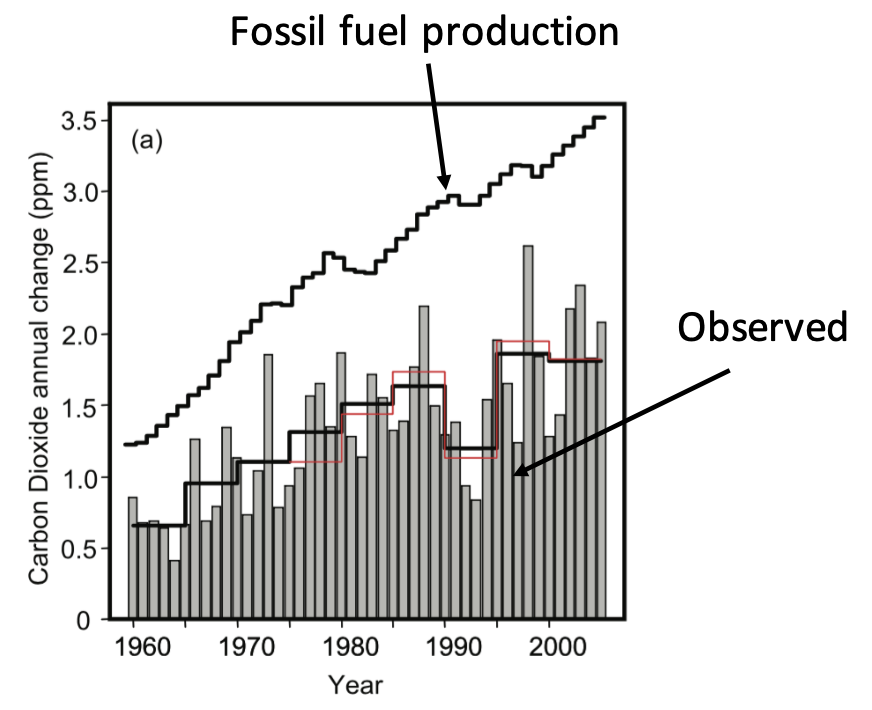
\includegraphics[width=\textwidth]{images/jeevanjee_human-caused-CO2_1.png}
\end{minipage} %
\hfill %
\begin{minipage}{0.48\textwidth}
\vspace{0pt}
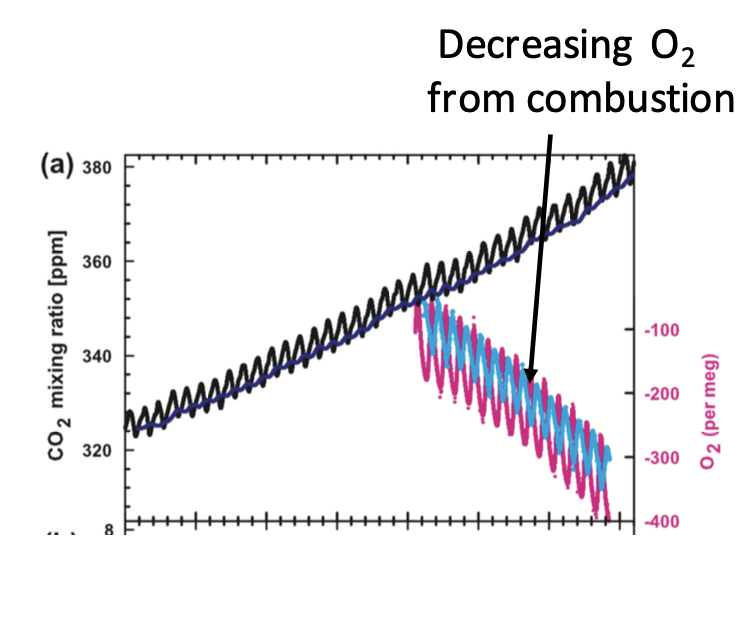
\includegraphics[width=\textwidth]{images/jeevanjee_human-caused-CO2_2.png}
\end{minipage}
\end{center}
%

% human production is sufficient

% some produced CO2 is not in atmosphere (absorbed by oceans, and plant mass)

\begin{itemize}
\item What does the comparison of human $\text{CO}_2$ production (line on left graph) and annual atmospheric increase (bars) tell us?
\item \underline{Combustion} is: $\text{C}_x \text{H}_y  + \text{O}_2 \rightarrow \text{H}_2 \text{O} + \text{CO}_2$
\end{itemize}

\vfill
{\tiny Sources: IPCC WG2 (Chapters 2 and 7)}

\end{frame}
%%%%%%%%%%%%%%%%%%%%%%%%%%%%%%%%%%%%%%
\begin{frame}{What about other effects, though?}

\begin{center}
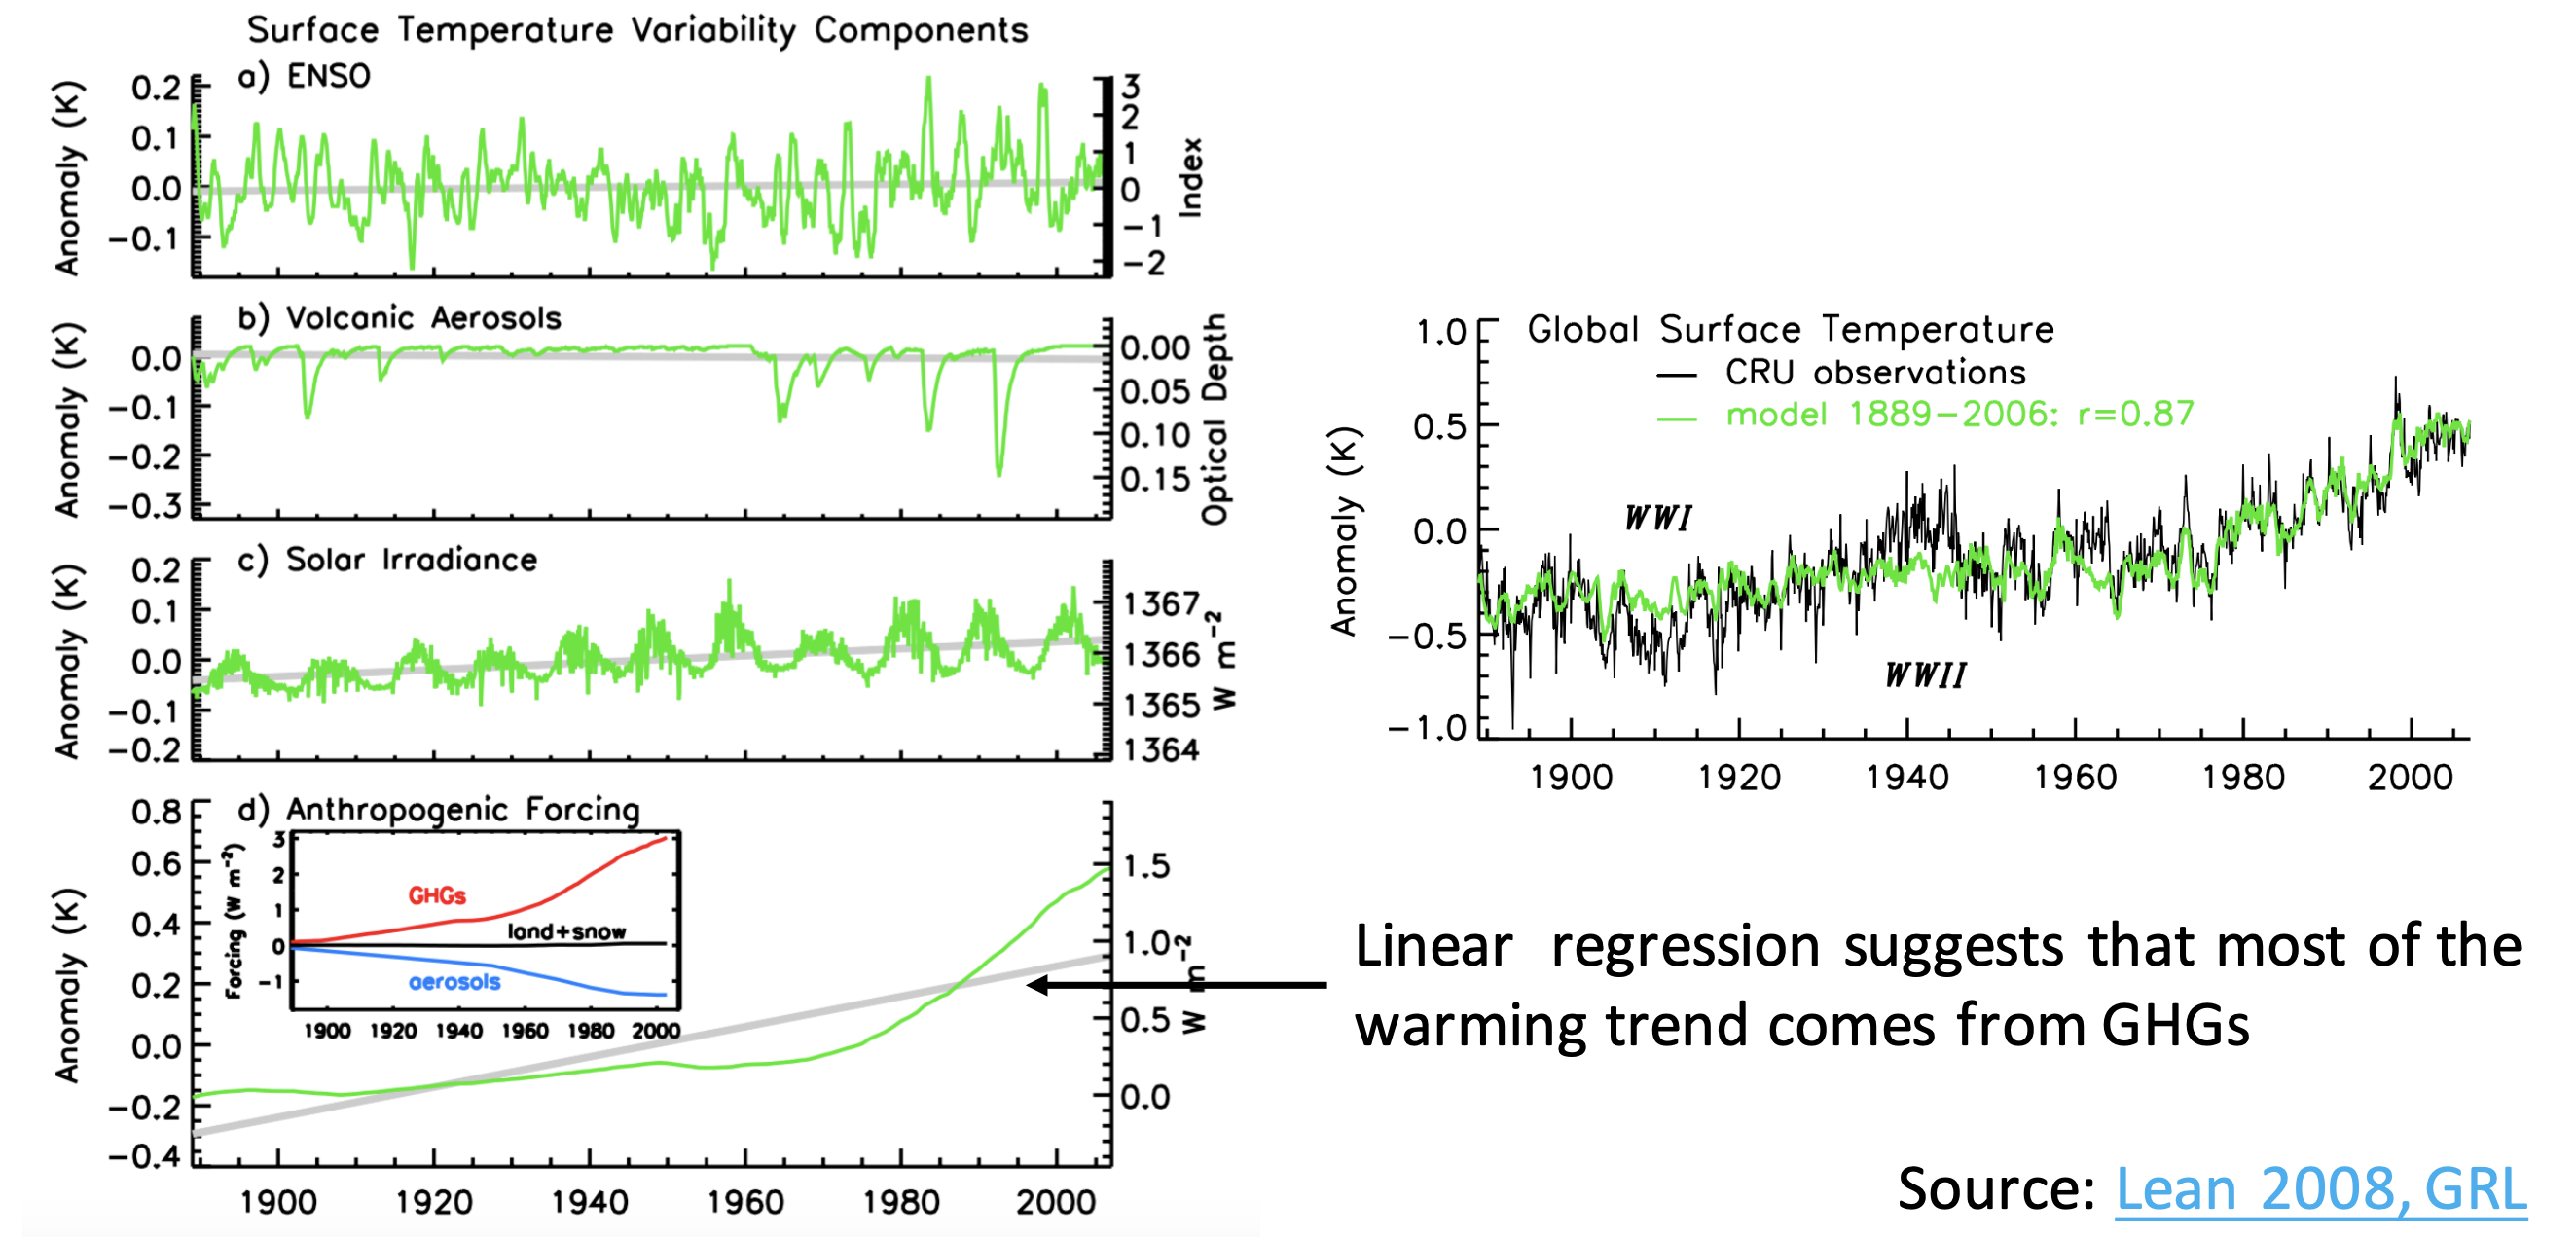
\includegraphics[width=\textwidth]{images/jeevanjee_forcings_slide8.png}
\end{center}
%

% human production is sufficient

% some produced CO2 is not in atmosphere (absorbed by oceans, and plant mass)

\begin{itemize}
\item Could solar variations explain warming?
\item Could natural ocean cycles (El Nino, La Nina)?
\item The effect of aerosols (causing cooling)?
\end{itemize}
\vfill
{\tiny (From Jeevanee talk)}
\end{frame}
%%%%%%%%%%%%%%%%%%%%%%%%%%%%%%%%%%%%%%
\begin{frame}{How do models take all of this into account?}

\begin{center}
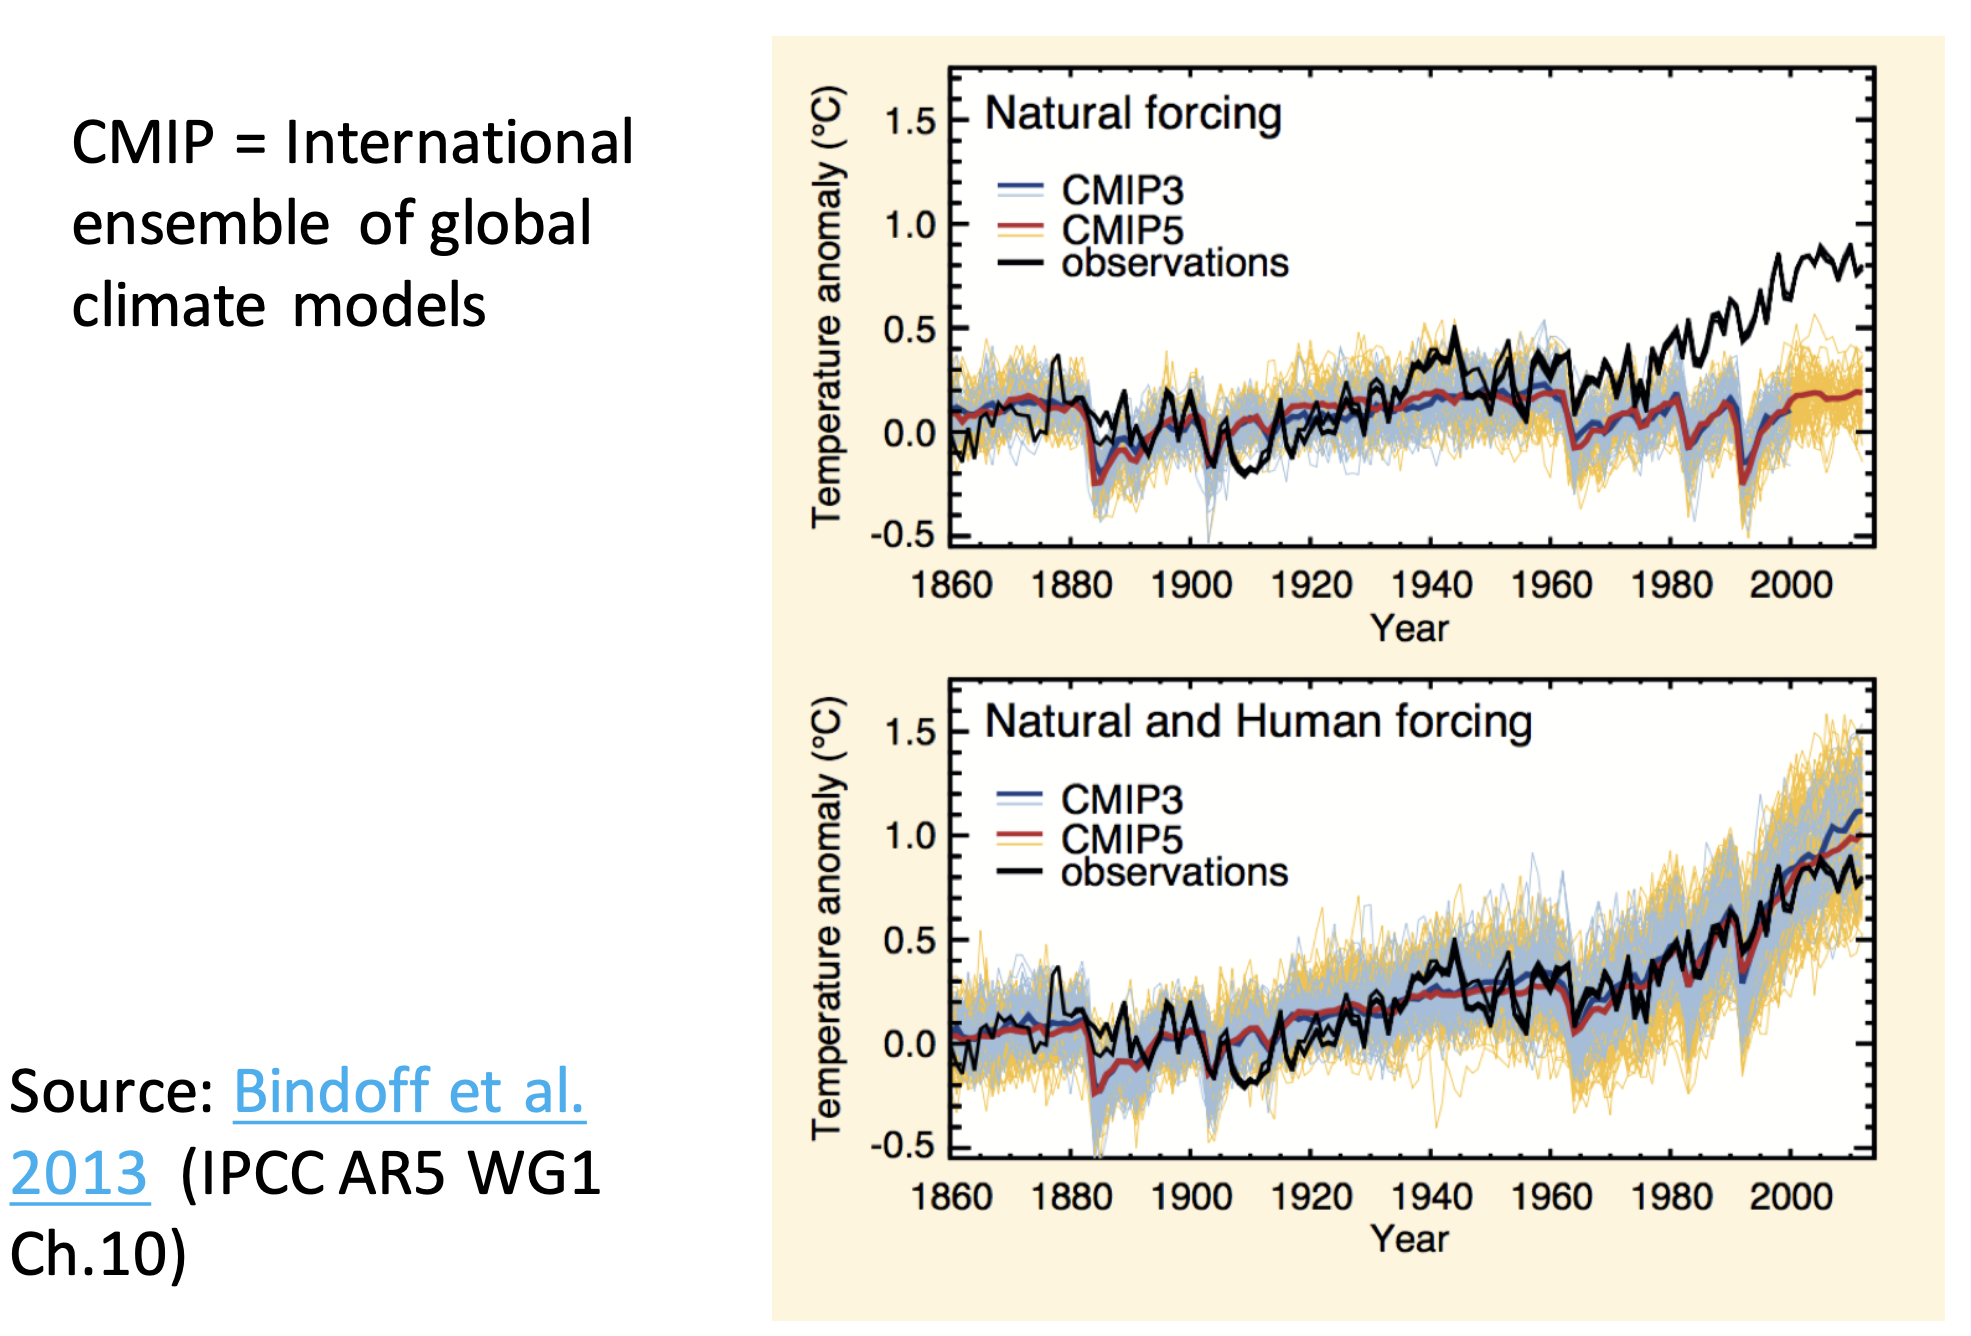
\includegraphics[width=0.95\textwidth]{images/jeevanjee_models_slide7.png}
\end{center}
%

% human production is sufficient

% some produced CO2 is not in atmosphere (absorbed by oceans, and plant mass)

\begin{itemize}
\item Models without human effects vs.\ those with.
\end{itemize}
\vfill
{\tiny (From Jeevanee talk)}
\end{frame}
%%%%%%%%%%%%%%%%%%%%%%%%%%%%%%%%%%%%%%
\begin{frame}{Different models agree on the contributing factors}

\begin{center}
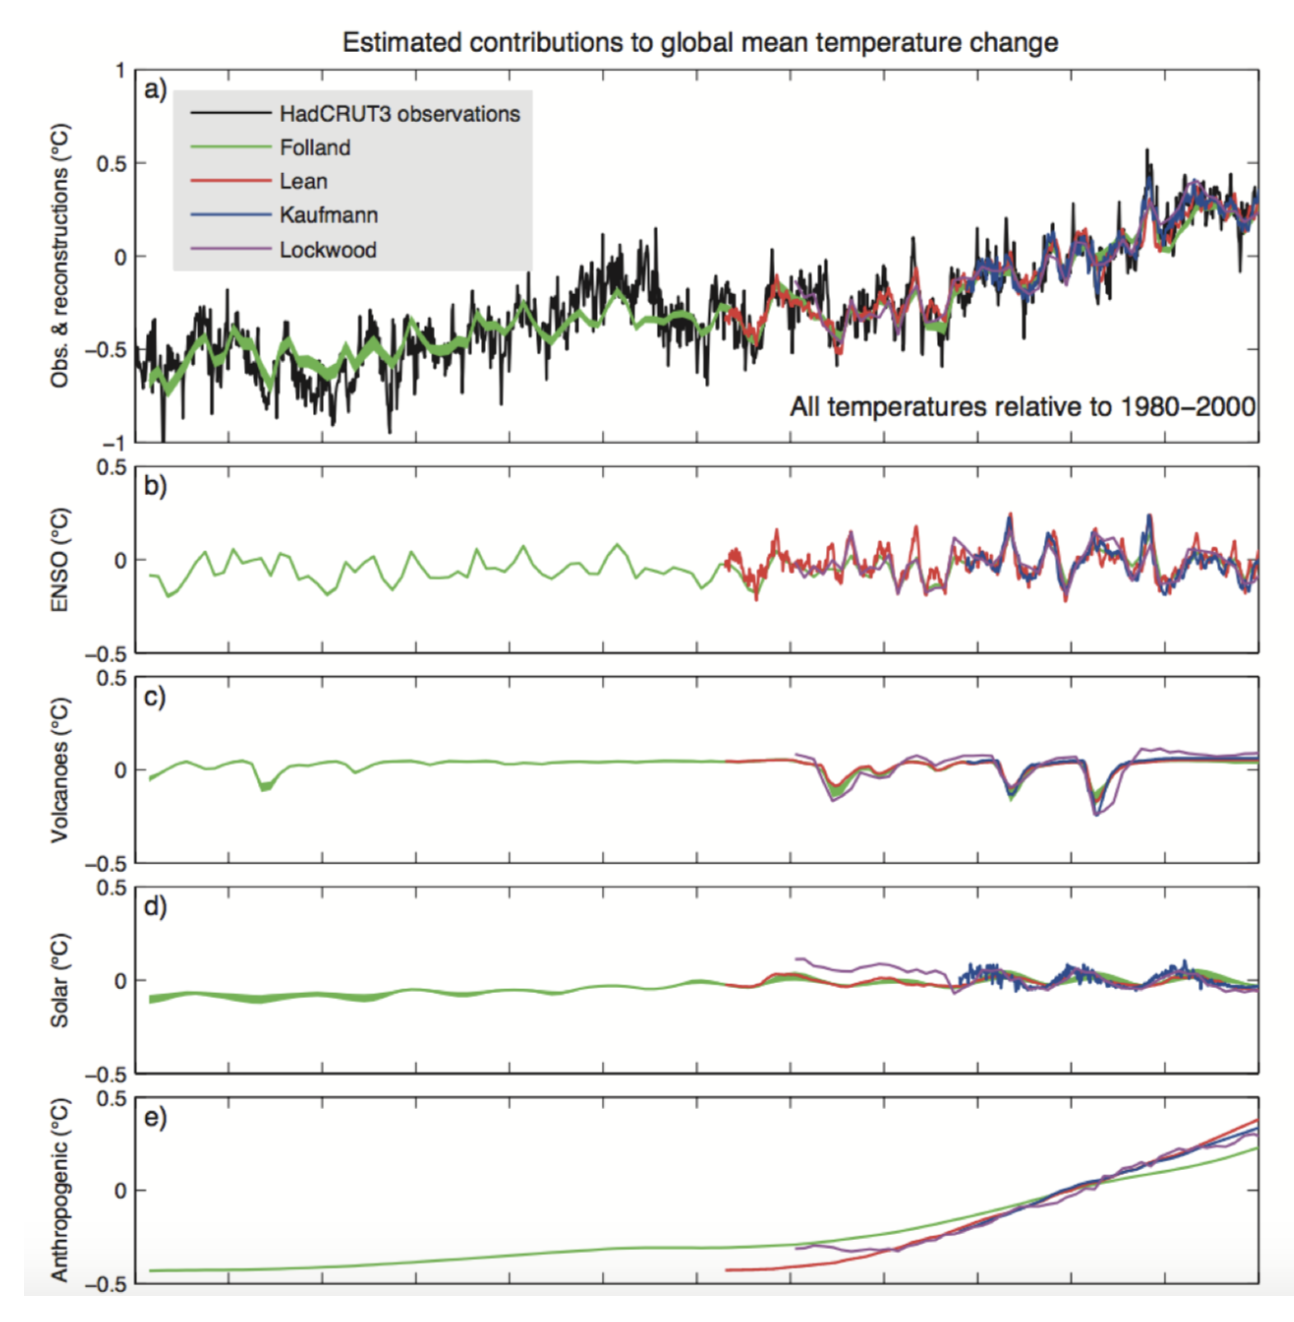
\includegraphics[width=0.7\textwidth]{images/jeevanjee_models-agree_slide9.png}
\end{center}
%


\vfill
{\tiny Sources: IPCC WG1 Chapter 10 (From Jeevanee talk)}
\end{frame}
%%%%%%%%%%%%%%%%%%%%%%%%%%%%%%%%%%%%%%
\begin{frame}{What do models predict for the future?}

\begin{center}
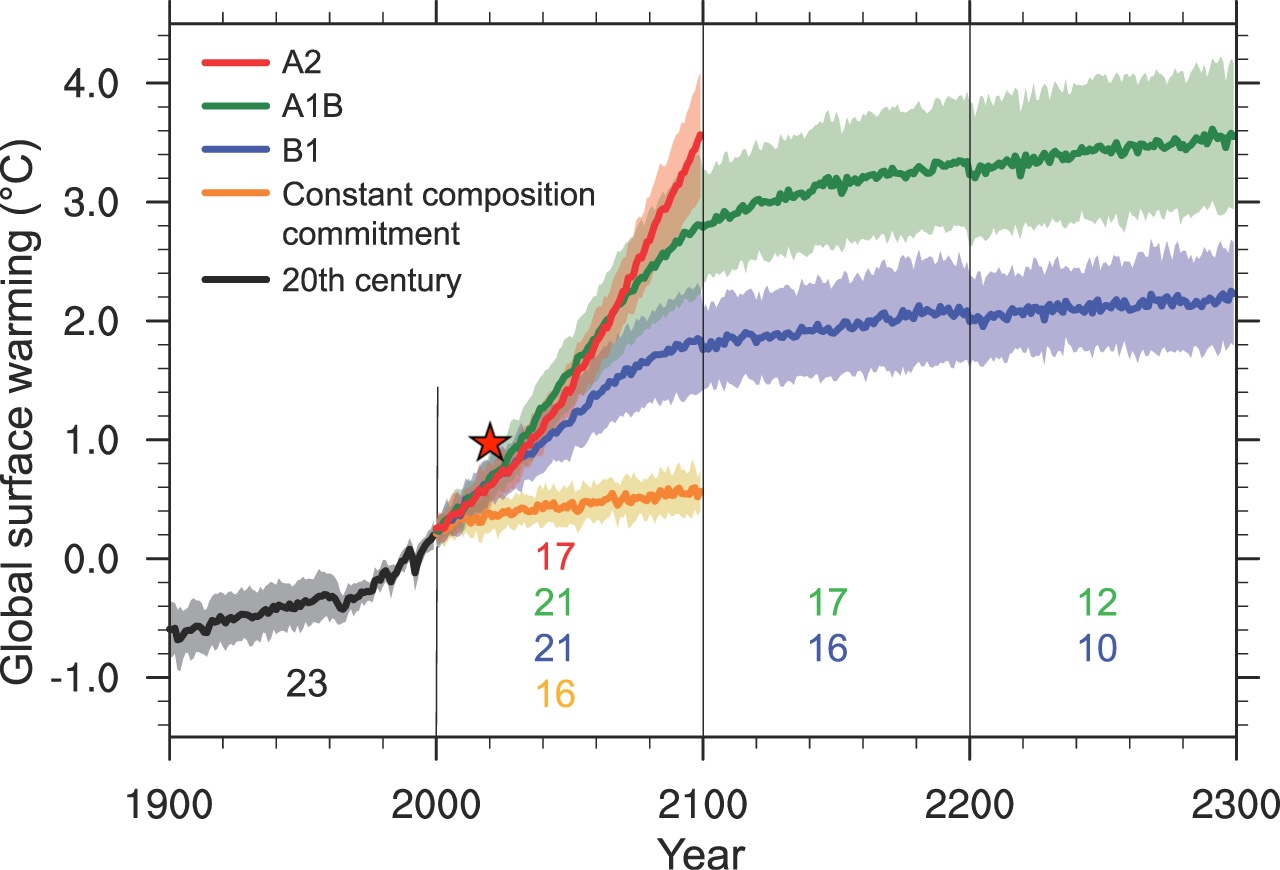
\includegraphics[width=0.9\textwidth]{images/ipcc-models-2007_fig-10-04-1_w-star.jpg}
\end{center}
%


\vfill
{\tiny Sources: IPCC Global Climate Predictions 2007 (Figure 10.4)}
\end{frame}
%%%%%%%%%%%%%%%%%%%%%%%%%%%%%%%%%%%%%%
\begin{frame}{What's in the news?}

\begin{center}
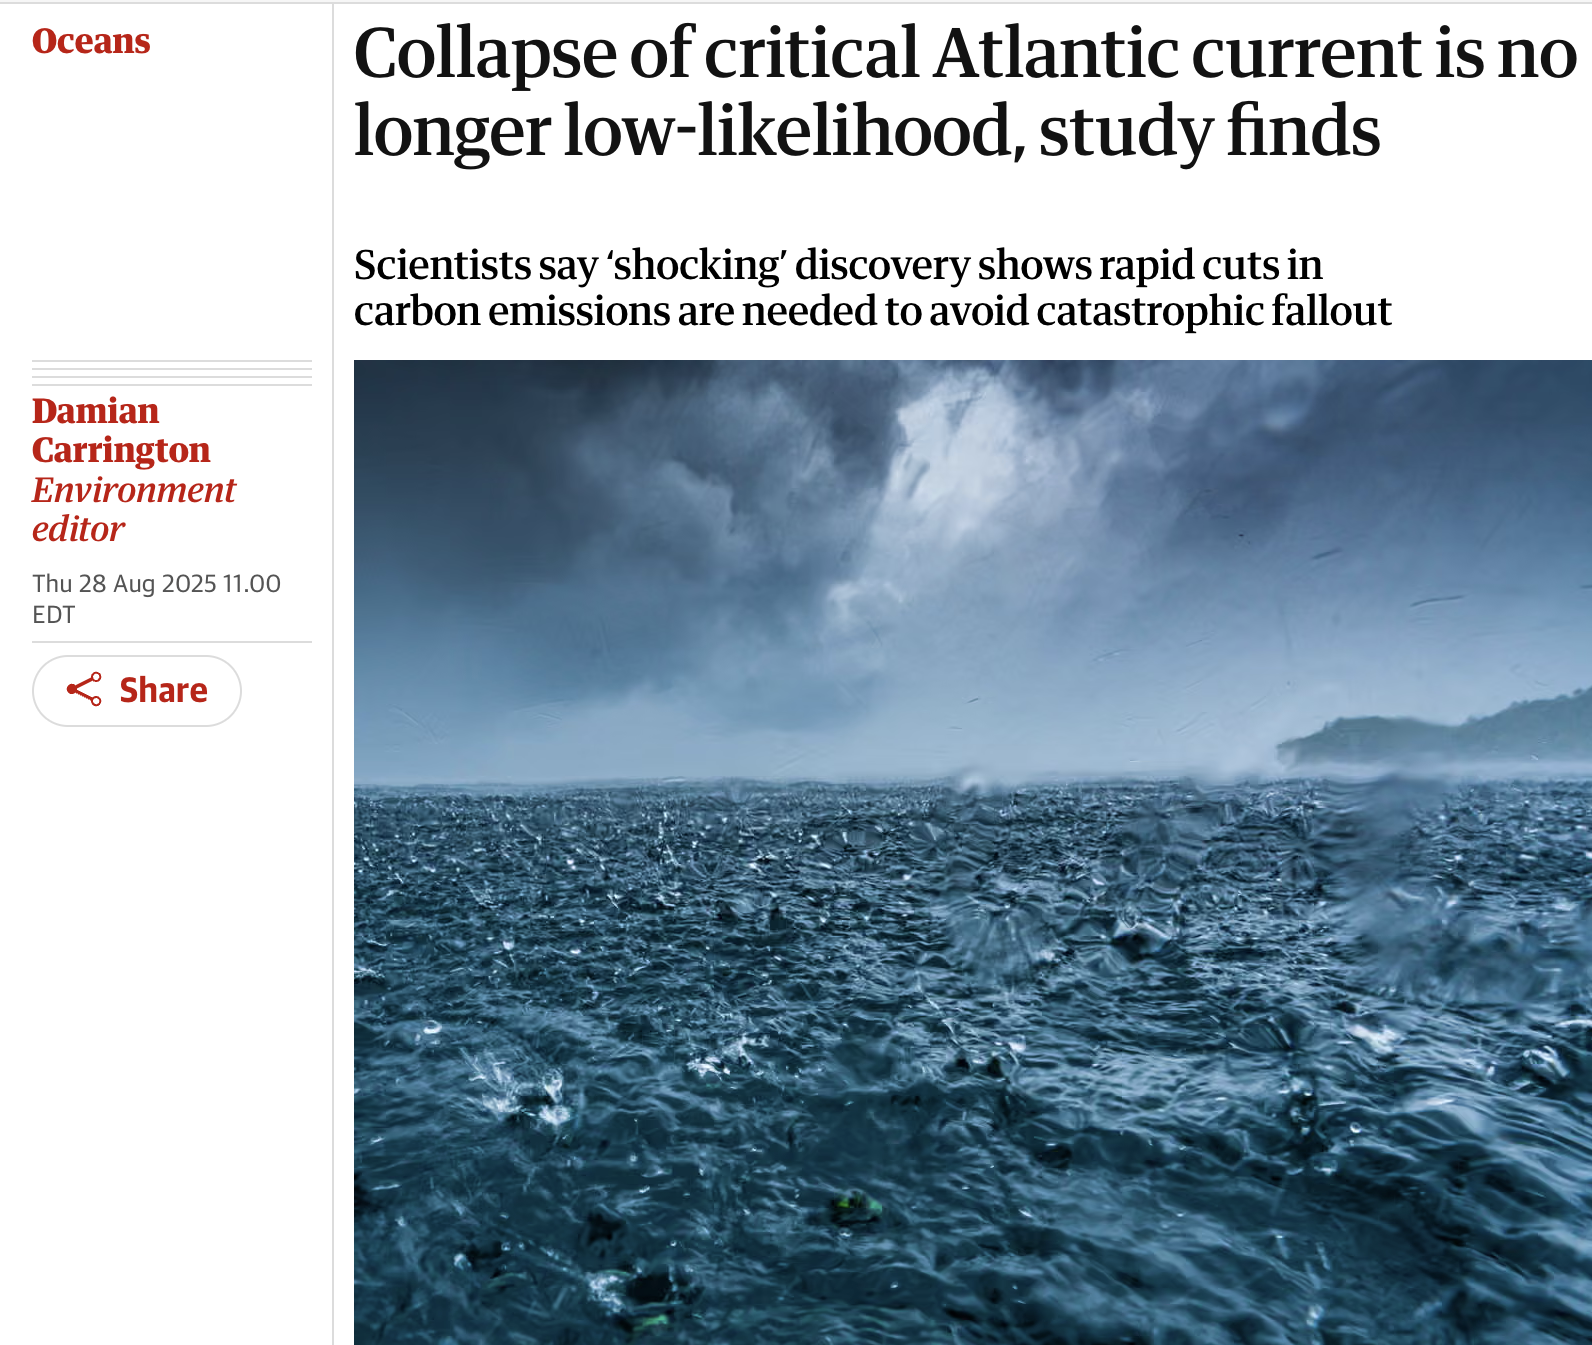
\includegraphics[width=0.9\textwidth]{images/guardian_2025-08-28_headline.png}
\end{center}
%


\vfill
{\tiny Sources: The Guardian, August 28, 2025}
\end{frame}
%%%%%%%%%%%%%%%%%%%%%%%%%%%%%%%%%%%%%%
\begin{frame}{AMOC}

\begin{center}
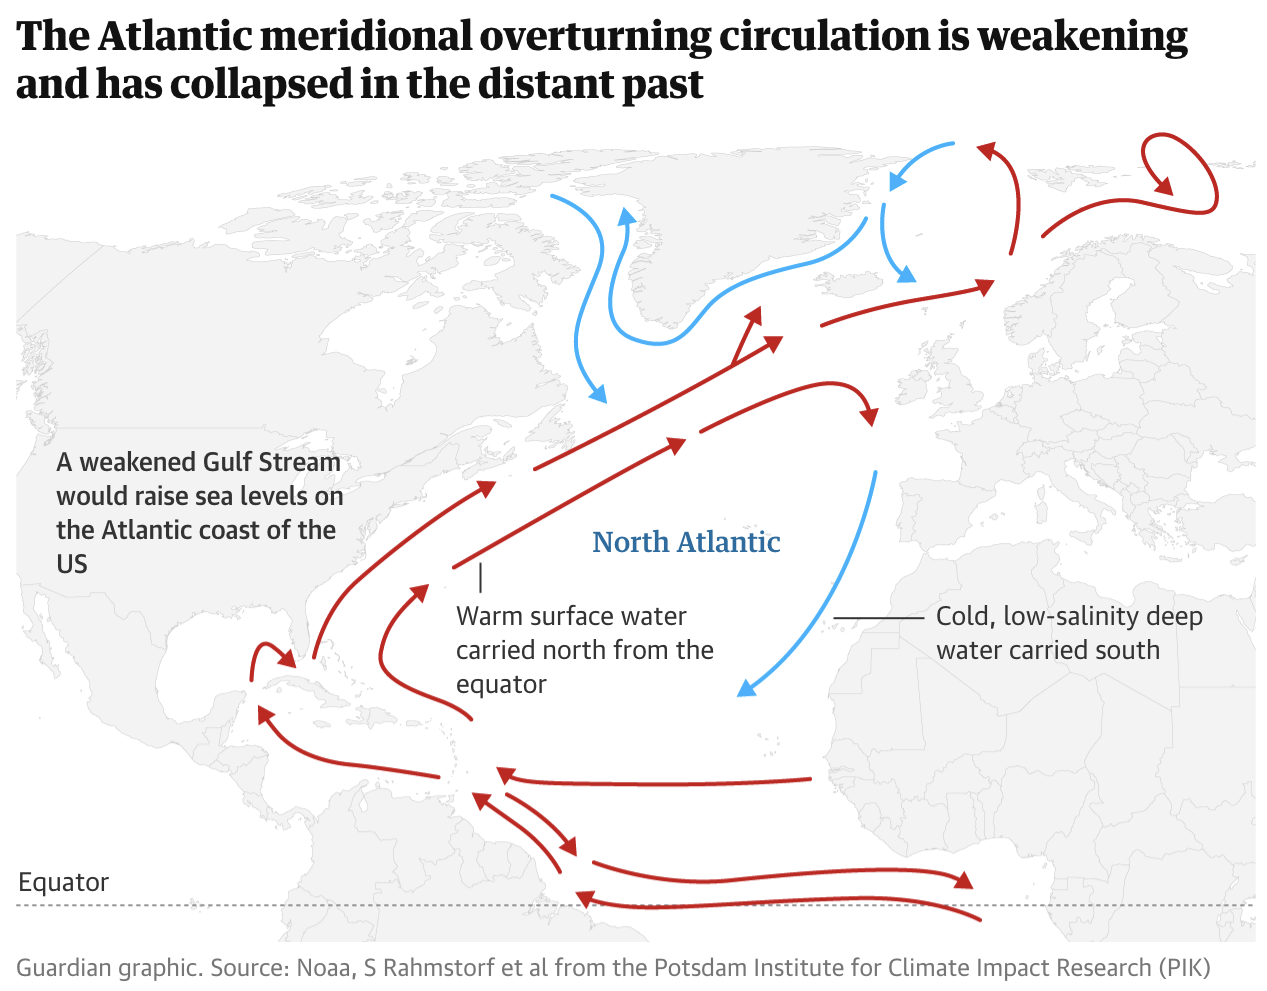
\includegraphics[width=0.9\textwidth]{images/guardian_2025-08_collapse-amoc.png}
\end{center}
%


\vfill
{\tiny Sources: The Guardian, August 28, 2025}
\end{frame}


%%%%%%%%%%%%%%%%%%%%%%%%%%%%%%%%%%%%%%
\end{document}
